\documentclass[a4paper,10pt,twoside]{article}

\usepackage[ngerman]{babel}
%\usepackage[top=3cm,bottom=3cm,left=3cm,right=3cm]{geometry} %NICHT IN KEMIE2


\usepackage{microtype} %schöneres typesetting  mit [stretch=10] für nur 1% anstelle von 2%
\usepackage{lmodern} %Latin Modern FONT
\usepackage{pifont} %schönere Font

\usepackage{chemfig}
\usepackage[version=4]{mhchem}
\usepackage{amsmath}
\usepackage{nicefrac}
\usepackage{amssymb}
%\usepackage{mathtools}

\usepackage{titlesec} %Um Section, etc bearbeiten zu können
\usepackage{fancyhdr}
\usepackage{setspace}
\usepackage{enumitem} %enumerate
\usepackage{arydshln} %für dashline
\usepackage{multicol}
\usepackage{lipsum}
\usepackage[labelfont=bf]{caption}

\usepackage[many]{tcolorbox}

%\usepackage{pgfornament} %Scheene Ornamente
\usepackage{witharrows} %Arrows in align-Umgebung
%\usepackage{awesomebox} %Notizboxen, etc
%\usepackage{textpos} %Für zum Beispiel vertikale Texte am Rand


%\usepackage{wrapfig} %Text um Bilder
%\usepackage{varwidth} % Alternative für engere minipage


\usepackage{hyperref}


\tcbuselibrary{theorems}

%\titlespacing*{\section}{0pt}{10mm}{3mm}
%\titlespacing*{\subsection}{0pt}{6mm}{3mm}
%\titlespacing*{\subsubsection}{0pt}{8mm}{3mm}


\renewcommand{\ttdefault}{lmtt} %Schriftart wird geändert zu Latin Modern Typewriter


\hypersetup{hidelinks,
			colorlinks=true,
			linkcolor=black,
			citecolor=miudiutex,
			urlcolor=miugray2
			}

\setlength\fboxsep{0pt}				
\setlength\columnsep{20pt}
\setlength{\parindent}{0pt}
\setcounter{section}{0}






%\definecolor{miudiutex}{HTML}{2f3d39}
\definecolor{miudiutex}{HTML}{1d2926}
\definecolor{miugray}{HTML}{b4cccf}
%\definecolor{miugray2}{HTML}{4d7365}
\definecolor{miugray2}{HTML}{6F8C81}
\definecolor{beige}{HTML}{F4F8D3}
\definecolor{white2}{HTML}{f5f7f8}
\definecolor{red}{HTML}{cf1f5c}
\definecolor{red2}{HTML}{9C191B}
\definecolor{green}{HTML}{00A36C}
\definecolor{delphinidin2}{HTML}{315794}
\definecolor{delphinidin}{HTML}{8B9EBA}
\definecolor{uniblau}{HTML}{004e9f}
\definecolor{unigelb}{HTML}{fcba00}
\definecolor{unigrau}{HTML}{909085}
\definecolor{pelargonidin}{HTML}{b33807}
\definecolor{pelargonidin2}{HTML}{FFDC96}
\definecolor{cyanidin}{HTML}{ba0746}
\definecolor{paeonidin}{HTML}{d15ca6}
\definecolor{petunidin}{HTML}{B88495}
\definecolor{petunitext}{HTML}{963354}
\definecolor{malvidin}{HTML}{8a2d8c}
\definecolor{mytheorembg}{HTML}{F2F2F9}
\definecolor{mytheoremfr}{HTML}{00007B}
\definecolor{uniblau2}{HTML}{27548A}
\definecolor{unigelb2}{HTML}{DDA853}
\definecolor{unidunkelblau2}{HTML}{183B4E}
\definecolor{unibeige}{HTML}{F5EEDC}


\tikzset{>=Latex}

\raggedcolumns %wichtig für Multicolumns
\color{miudiutex}



\usetikzlibrary{chains,
                positioning,
                shapes.multipart,
                }


\setchemfig
{%	
	bond offset=2pt,
	atom sep=15pt, 
	cram width=3pt,
	cram dash width=0.8pt,
	cram dash sep=1.2pt,
	double bond sep=2.5pt, 
	bond style={line width=1.1pt,cap=round},
	baseline=(current bounding box.center),
	bond join=true
}
\setcharge{extra sep=3pt}





%================================
% SYMBOLS
%================================

\newcommand{\RA}{$\rightarrow$~}
\newcommand{\RL}{$\rightleftharpoons$~}
\newcommand{\HARP}{\ding{226}~}
%$\xrightarrow{2}$ %Pfeil mit 2 drüber


%================================
% SHORT COMMANDS (BOXES ; ETC)
%================================


\newcommand{\info}[1]{\begin{note}{\color{miudiutex}#1}\end{note}}
\newcommand{\qsbig}[1]{\begin{qstion}{}{}\begin{center}
			#1 \end{center}\end{qstion}}
\newcommand{\notiz}[1]{\begin{notizz}{}{}\begin{center}
			{\color{miugray2!50!miudiutex}#1} \end{center}\end{notizz}}
\newcommand{\klausur}[1]{\begin{klausurinfo}{}{}\begin{center}
			#1 \end{center}\end{klausurinfo}}
\newcommand{\dfn}[1]{\begin{defin}{}{}\begin{center}
			#1 \end{center}\end{defin}}
\newcommand{\gesetz}[2]{\begin{gestex}{}{}\begin{center}
			#1 \end{center}\end{gestex}}
\newcommand{\gergesetz}[1]{\begin{gesgex}{}{}\begin{center}
			#1 \end{center}\end{gesgex}}
\newcommand{\klaausur}[1]{\begin{klausurinfo}[width=.77\linewidth]{}{}\begin{center}
			\footnotesize #1 \end{center}\end{klausurinfo}}
\newcommand{\winfo}[1]{\begin{wichtig}{}{} \begin{center}
#1 \end{center} \vspace*{0mm} \end{wichtig}}
\newcommand{\zit}[2]{\begin{zitat}{#1}{}\small #2 \end{zitat}}



\newcommand{\unten}{\end{center} \tcblower \begin{center}}


\newcommand*\circled[1]{\tikz[baseline=(char.base)]{
            \node[shape=circle,draw,inner sep=0.5pt,miudiutex] (char) {\tiny #1};}}
            
\newcommand{\miusquare}{{\color{miugray2!50}\scriptsize $\blacksquare$}~}
\newcommand{\miusquarp}{{\color{petunidin!50}\scriptsize $\blacktriangleright$}~}
\newcommand{\niu}{\item[\miusquare]}
\newcommand{\nip}{\item[\miusquarp]}
\newcommand{\mrk}[1]{{\color{petunitext!55!red}\textsc{#1}}}

%%%%% ABSAETZE

\newcommand{\pps}{\par \vspace*{1mm}}
\newcommand{\pp}{\par \vspace*{3mm}}
\newcommand{\ppbig}{\par \vspace*{8mm}}
\newcommand{\pphuge}{\par \vspace*{10mm}}



%================================
% HEADER & FOOTER FUER UNI
%================================
\newcommand{\miusfoot}{
\fancypagestyle{plain}{%
  \fancyhf{}%
  \renewcommand{\footrulewidth}{0.0mm}%
  \fancyfoot[L]{\hspace*{-3cm} {\color{miugray2}\textbf{\thepage}}}%
  \renewcommand{\headrulewidth}{0mm}%
} 
\pagestyle{plain}
}

\newcommand{\miushead}[2]{
\miusquare #1 - 4.Semester - ELW \hfill 
\includegraphics[width=60pt]{{F://LaTeX-Files/shiet/unibo}}
\par \vspace*{-3mm}
\hrulefill
\par \vspace*{1mm}
\par \vspace*{-4mm}
\normalsize	
	\begin{flushright}
	\textbf{\miusquare #2}\par \vspace*{1.5mm}
	\small	
	\textit{Letzte Überarbeitung:} \par 
	\footnotesize \today
	\end{flushright}
	\normalsize
\par \vspace*{-8mm}
}

\newcommand{\sidebar}{
\AddToHook{shipout/background}{
  \begin{tikzpicture}[remember picture,overlay, shift={(current page.south west)}]
   \path[fill=miugray2!15](0,0) rectangle (3.5cm,\paperheight);
%   \path[fill=miugray2!8](0,0) rectangle (3.5cm,\paperheight);
   \path[draw,miudiutex!50] (3.5,0) to (3.5,\paperheight);
%   \path[draw,miudiutex!50,dashed] (3.5,0) to (3.5,\paperheight);  
%   \node[opacity=0.8](a)at(12,10){\includegraphics[width=9cm]{F://LaTeX-Files/pngs/girl01}};
  \end{tikzpicture} 
}
}


\newcommand{\oddsidebar}{
\AddToHook{shipout/background}{
   \put(0in,-\paperheight){%
      \ifodd\value{page}\relax
           \begin{tikzpicture}[remember picture,overlay, shift={(current page.south west)}]
   \path[fill=miugray2!15](0,0) rectangle (3.5cm,\paperheight);
      \path[draw,miudiutex!50] (3.5,0) to (3.5,\paperheight);
  \end{tikzpicture}
      \else
           \begin{tikzpicture}[remember picture,overlay, shift={(current page.south east)}]
   \path[fill=miugray2!15](-3,0) rectangle (3cm,\paperheight);
%      \path[draw,miudiutex!50] (-3.5,0) to (-3.5,\paperheight);
  \end{tikzpicture}
      \fi
   }
}
}
%================================
% ENVIRONMENTS
%================================

\newenvironment{ctab}[2]{%
				\begin{spacing}{#1}
					\begin{center}
					\begin{tabular}{#2}}
					{\end{tabular}
					\end{center}
				\end{spacing}
				}


%================================
% Farbiger-Background-Box
%================================



\newcommand{\farbig}[1]{
\begin{tcolorbox}[%
				hbox,
				colback=miugray2!25,
				boxsep=-2pt,
				boxrule=0pt,
				arc=0pt,
				nobeforeafter,
				tcbox raise base,
				shrink tight,
				extrude by=1pt
				]
				{\color{miudiutex}{#1}}
\end{tcolorbox}~}

%================================
% SIMPLE SCHWARZER RAHMEN BOX
%================================


\newcommand{\boxfr}[1]{
	\begin{tcolorbox}[
	colframe=miugray2,
	colback=white!95!miugray2,
	boxrule = 0.5pt, 
%	toprule=0pt, bottomrule=0pt,rightrule=0pt,leftrule=0pt,
	boxsep=0pt,
	arc=4pt,
	drop shadow southeast,
	enhanced
	]
	\color{miudiutex}
	\begin{center}
	#1
	\end{center}
	\end{tcolorbox}
}

%================================
% Antwort-Box
%================================

\newcommand{\antwort}[1]{\par 
	\begin{tcolorbox}[
	colback=gray!15,
	breakable,
	enhanced,
	frame hidden,
	arc=5pt,
	boxrule = 2pt,
%	borderline west = {2pt}{0pt}{petunidin},
%	drop shadow=miugray2!30
	]
	\color{miudiutex}	#1
	\end{tcolorbox}
}

%================================
% Frame-IT
%================================

\newcommand{\frameit}[1]{\par 
	\begin{tcolorbox}[
	colback=gray!10,
	breakable,
	enhanced,
	frame hidden,
	arc=5pt,
	boxrule = 0pt,
	borderline west = {4pt}{0pt}{petunidin},
%	drop shadow=miugray2!30
	]
		#1
	\end{tcolorbox}
}



%================================
% Question BOX
%================================

\makeatletter
\newtcbtheorem{qstion}{Frage}{enhanced,
	breakable,
	colback=white,
	colframe=delphinidin!100,
%	capture=hbox,
	boxsep=-3pt,
	attach boxed title to top left={yshift*=-\tcboxedtitleheight},
	fonttitle=\bfseries,
%	title={#2},
	boxed title size=title,
	boxed title style={%
			sharp corners,
			rounded corners=northwest,
			colback=tcbcolframe,
			boxrule=0pt,
		},
	underlay boxed title={%
			\path[fill=tcbcolframe] (title.south west)--(title.south east)
			to[out=0, in=180] ([xshift=5mm]title.east)--
			(title.center-|frame.east)
			[rounded corners=\kvtcb@arc] |-
			(frame.north) -| cycle;
		},
	#1
}{def}
\makeatother



%================================
% SIMPLE Question BOX
%================================

\newcommand{\qssmall}{
\begin{tcolorbox}[hbox,colback=miugray2!55,boxsep=-4pt,boxrule=0pt,arc=2pt,nobeforeafter, tcbox raise base,shrink tight,extrude by=3pt]
\textbf{\color{white}{?}}
\end{tcolorbox}~~}

\newcommand{\folie}[1]{
\begin{tcolorbox}[%
				hbox,
				colback=miugray2!20,
				boxsep=2pt,
				boxrule=0.5pt,
				arc=2pt,
				nobeforeafter,
				tcbox raise base,
				shrink tight,
				extrude by=3pt]
				{\color{miudiutex}{Folie #1}}
\end{tcolorbox}~}


%================================
% NOTIZ BOX
%================================

\makeatletter
\newtcbtheorem{notizz}{Notiz}{enhanced,
	breakable,
	coltitle=white,
	colback=petunidin!10,
	colframe=petunidin!50,
	attach boxed title to top left={yshift*=-\tcboxedtitleheight},
	fonttitle=\bfseries,
%	title={#2},
	boxed title size=title,
	boxed title style={%
			sharp corners,
			rounded corners=northwest,
			colback=tcbcolframe,
			boxrule=0pt,
		},
	underlay boxed title={%
			\path[fill=tcbcolframe] (title.south west)--(title.south east)
			to[out=0, in=180] ([xshift=5mm]title.east)--
			(title.center-|frame.east)
			[rounded corners=\kvtcb@arc] |-
			(frame.north) -| cycle;
		},
		#1
}{def}
\makeatother



%================================
% Question BOX: Klausur
%================================

\makeatletter
\newtcbtheorem[no counter]{klausurinfo}{Klausurrelevant}{enhanced,
%	breakable,
	colback=miugray2!10,
	colframe=miugray2!75,
	attach boxed title to top left={yshift*=-\tcboxedtitleheight},
	fonttitle=\bfseries,
	title={#2},
	arc=4pt,
	boxrule=1pt,
	boxed title size=title,
	boxed title style={%
			sharp corners,
			rounded corners=northwest,
			colback=tcbcolframe,
			boxrule=0pt,
			arc=4pt,
		},
	underlay boxed title={%
			\path[fill=tcbcolframe] (title.south west)--(title.south east)
			to[out=0, in=180] ([xshift=5mm]title.east)--
			(title.center-|frame.east)
			[rounded corners=\kvtcb@arc] |-
			(frame.north) -| cycle;
		},
	#1
}{def}
\makeatother


%================================
% DEFINITION
%================================

\makeatletter
\newtcbtheorem[no counter]{defin}{Definition}{enhanced,
	breakable,
	colback=gray!10,
	colframe=gray,
	attach boxed title to top left={yshift*=-\tcboxedtitleheight},
	fonttitle=\bfseries,
	title={#2},
	arc=4pt,
	boxrule=1pt,
	fontlower=\footnotesize,
	collower=miugray2!50!miudiutex,
	boxed title size=title,
	boxed title style={%
			sharp corners,
			rounded corners=northwest,
			colback=tcbcolframe,
			boxrule=0pt,
			arc=4pt,
		},
	underlay boxed title={%
			\path[fill=tcbcolframe] (title.south west)--(title.south east)
			to[out=0, in=180] ([xshift=5mm]title.east)--
			(title.center-|frame.east)
			[rounded corners=\kvtcb@arc] |-
			(frame.north) -| cycle;
		},
	#1
}{def}
\makeatother

%================================
% Gesetzes-Text EU
%================================

\makeatletter
\newtcbtheorem[no counter]{gestex}{EU - Verordnung}{enhanced,
	breakable,
	colback=gray!10,
	colframe={gray!65!delphinidin},
	attach boxed title to top left={yshift*=-\tcboxedtitleheight},
	fonttitle=\bfseries,
	arc=4pt,
	boxsep=10pt,
	boxrule=1pt,
	fontlower=\footnotesize,
	collower=miugray2!50!miudiutex,
	boxed title size=title,
	overlay={%
			\node[xshift=-1cm,yshift=-1mm] at (frame.north east)
			{\includegraphics[width=8mm]{F://LaTeX-Files/shiet/eu}};
%			\node[draw,miugray2] at (frame.north) {{#2}}; 
			},%
	boxed title style={%
			sharp corners,
			rounded corners=northwest,
			colback=tcbcolframe,
			boxrule=0pt,
			arc=4pt,
		},
	underlay boxed title={%
			\path[fill=tcbcolframe] (title.south west)--(title.south east)
			to[out=0, in=180] ([xshift=5mm]title.east)--
			(title.center-|frame.east)
			[rounded corners=\kvtcb@arc] |-
			(frame.north) -| cycle;
		},
	#1
}{def}
\makeatother


%================================
% Gesetzes-Text Ger
%================================

\makeatletter
\newtcbtheorem[no counter]{gesgex}{Gesetzestext}{enhanced,
	breakable,
	colback=gray!10,
	colframe={gray!95!pelargonidin},
	attach boxed title to top left={yshift*=-\tcboxedtitleheight},
	fonttitle=\bfseries,
	title={#2},
	arc=4pt,
	boxrule=1pt,
	fontlower=\footnotesize,
	collower=miugray2!50!miudiutex,
	boxed title size=title,
	overlay={\node[xshift=-1cm,yshift=-3mm] at (frame.north east)
			{\includegraphics[width=8mm]{F://LaTeX-Files/shiet/ger}}; 
			},
	boxed title style={%
			sharp corners,
			rounded corners=northwest,
			colback=tcbcolframe,
			boxrule=0pt,
			arc=4pt,
		},
	underlay boxed title={%
			\path[fill=tcbcolframe] (title.south west)--(title.south east)
			to[out=0, in=180] ([xshift=5mm]title.east)--
			(title.center-|frame.east)
			[rounded corners=\kvtcb@arc] |-
			(frame.north) -| cycle;
		},
	#1
}{def}
\makeatother


%================================
% Question BOX: Wichtig
%================================

%\makeatletter
%\newtcbtheorem[no counter]{wichtig}{Wichtige Info}{enhanced,
%	breakable,
%	colback=pelargonidin2!80,
%	colframe=red2!100,
%	fonttitle=\bfseries,
%	title={#2},
%	leftrule=5mm,
%	boxed title size=title,
%	boxed title style={%
%			sharp corners,
%			rounded corners=northwest,
%			colback=tcbcolframe,
%			boxrule=0pt,
%		},
%	underlay boxed title={%
%			\path[fill=tcbcolframe] (title.south west)--(title.south east)
%			to[out=0, in=180] ([yshift=1mm,xshift=7mm]title.east)--
%			([yshift=1mm]title.center-|frame.east)
%			[rounded corners=\kvtcb@arc] |-
%			(frame.north) -| cycle;
%		},
%		watermark tikz={\draw[line width=2mm] circle (1.1cm)
%		node{\fontfamily{ptm}\fontseries{b}\fontsize{20mm}{20mm}\selectfont !};}],
%	attach boxed title to top left={xshift=5mm,yshift*=-\tcboxedtitleheight},
%	watermark zoom=0.65,
%	  underlay={%
%    \path[draw=none] (interior.south west) rectangle node[white]{\Huge \textbf{!}} ([xshift=-4mm]interior.north west);
%    },
%	#1
%}{def}
%\makeatother


\makeatletter
\newtcbtheorem[no counter]{wichtig}{Wichtige Info}{enhanced,
	breakable,
	colback=pelargonidin2!30,
	colframe=petunidin!100,
	fonttitle=\footnotesize\bfseries,
	title={#2},
	leftrule=4mm,
	boxed title size=title,
	boxed title style={%
			sharp corners,
			rounded corners=northeast,
			colback=tcbcolframe,
			boxrule=0pt,
		},
	underlay boxed title={%
			\path[fill=tcbcolframe] (title.south east)--(title.south west)
			to[out=180, in=0] ([yshift=2mm,xshift=-7mm]title.west)--
			([yshift=2mm]title.center-|frame.west)
			[rounded corners=\kvtcb@arc] |-
			(frame.north) -| cycle;
		},
		watermark tikz={\draw[line width=2mm] circle (1.1cm)
		node{\fontfamily{ptm}\fontseries{b}\fontsize{20mm}{20mm}\selectfont !};},
	attach boxed title to top right={yshift*=-\tcboxedtitleheight},
	watermark zoom=1.45,
	watermark opacity=0.35,
	  underlay={%
    \path[draw=none] (interior.south west) rectangle node[white]{\LARGE \textbf{!}} ([xshift=-4.3mm]interior.north west);
    },
    #1
}{def}
\makeatother





%================================
% ZITAT BOX
%================================

\tcbuselibrary{theorems,skins,hooks}
\newtcbtheorem{zitat}{Zitat}
{%
	enhanced,
	breakable,
	colback = gray!10!white,
	frame hidden,
	boxrule = 0sp,
	borderline west = {2pt}{0pt}{petunidin},
	sharp corners,
	detach title,
	before upper = \tcbtitle\par\smallskip,
	coltitle = gray!50!black,
	fonttitle = \bfseries\sffamily,
	description font = \mdseries,
	separator sign none,
	segmentation style={solid, gray!50!black},
}
{th}



%\usepackage[top=2cm,bottom=2cm,left=4cm,right=2cm,heightrounded,
%  marginparwidth=2.7cm, marginparsep=8mm]{geometry}
%  \usepackage[top=2cm,bottom=2cm,left=2cm,right=1cm,heightrounded,
%  marginparwidth=0.7cm, marginparsep=8mm]{geometry}
\usepackage[top=3cm,bottom=3cm,left=3cm,right=3cm,heightrounded]{geometry}
\usepackage{awesomebox}
\usepackage{marginnote}
%\setcounter{secnumdepth}{0}
\usepackage{letltxmacro}



\usepackage[strict]{changepage}
\usepackage{refcount}
\usepackage{titletoc}
\usepackage{tikzpagenodes}
\usetikzlibrary{calc}
\usetikzlibrary{patterns.meta}
\usetikzlibrary{calc,shapes.symbols,decorations.pathreplacing}



\colorlet{mycolor}{petunitext}
\colorlet{myc2}{miugray2!50!miudiutex}




\titlecontents{section}%
 	 	[10mm]
 	 	{\vspace{1.5\baselineskip} \large \sffamily \bfseries \color{myc2}}
 	 	{\hspace*{0em}\llap{\parbox[t]{40pt}{\hfill\color{mycolor}\thecontentspage}\hspace*{10pt}}}
 	 	{\thecontentspage}
 	 	{\sffamily \qquad }

\titlecontents{subsection}%
	 	 [12mm]
	  	{\vspace{.3\baselineskip}\normalsize \sffamily \color{myc2}}
	  	{\hspace*{0em}\llap{\parbox[t]{40pt}{\hfill\color{mycolor}\thecontentspage}\hspace*{10pt}}}
	  	{\thecontentspage}
 	 	{\sffamily\qquad}

\titlecontents{subsubsection}%
 	 	[14mm]
	 	{\vspace{.3\baselineskip}\normalsize \sffamily \color{myc2}}
 		{\hspace*{0em}\llap{\parbox[t]{40pt}{\hfill\color{mycolor}\thecontentspage}\hspace*{10pt}}}
	  	{\thecontentspage}
	  	{\sffamily\qquad}




\titlespacing*{\section}{0pt}{30mm}{6mm}
\titlespacing*{\subsection}{0pt}{18mm}{3mm}
\titlespacing{\subsection}{0pt}{12mm}{3mm}
\titlespacing*{\subsubsection}{0pt}{6mm}{3mm}
\titlespacing{\subsubsection}{0pt}{6mm}{2mm}
\titlespacing{\paragraph}{0pt}{6mm}{2mm}



\titleformat{\section}[hang]
		{\LARGE \sffamily \bfseries \color{miudiutex!80!miugray2}}
		{\thesection}
		{4mm}
		{}

\titleformat{\subsection}[hang]
		{\large \sffamily \bfseries \color{miudiutex!50!miugray2}}
		{\thesubsection}
		{4mm}
		{}

\titleformat{\subsubsection}[block]
		{\normalsize \bfseries \sffamily \color{miudiutex!50!miugray2}}%
		{\normalsize \color{petunitext} \thesubsubsection}
		{2mm}
		{}
		[ \color{miugray}{\titlerule[0.3pt]}]
		
\titleformat{\paragraph}
		{\large \bfseries \sffamily \color{petunitext}}
		{\footnotesize \theparagraph}
		{1mm}
		{}



\renewcommand*{\marginfont}{\scriptsize\color{miudiutex!30!miugray2}\sffamily}
\renewcommand{\textbf}[1]{\textsf{{\bfseries {#1}}}}
\renewcommand{\labelitemi}{\miusquare}
\renewcommand{\labelitemii}{\miusquarp}
\setitemize{itemsep=0pt,labelsep=5pt,leftmargin=20pt}
\LetLtxMacro\mn\marginnote







\usepackage{awesomebox}
\usepackage{pgfplots}
\usepackage{booktabs, makecell}
\usepackage{caption}
\usepackage{hypcap}
\usepackage[makeroom]{cancel}
\usepackage{sidenotes}

\usepackage[labelfont={bf},font={color=miudiutex,small},figurename={\miusquare $~$Abbildung}]{caption}


\usepgfplotslibrary{fillbetween}
\usetikzlibrary{patterns.meta}
\usetikzlibrary{calc,shapes.symbols,decorations.pathreplacing}

\tikzset{
  mynode/.style={
    draw, execute at begin node=\setlength{\baselineskip}{12pt}
  },
  every pin/.style={fill=miugray2!40!white,rectangle,rounded corners=3pt,font=\tiny},
  small dot/.style={fill=black,circle,scale=0.3}
}

%\setcounter{section}{1} % <--- FALLS KEINE SECTION DEFINIERT WIRD










\newgeometry{top=2cm,bottom=2cm,left=6cm,right=2.cm,marginparsep=0.5cm,marginparwidth=4.5cm}
\counterwithin{equation}{section}


\let\oldmarginfigure\marginfigure
\let\endoldmarginfigure\endmarginfigure

\renewenvironment{marginfigure}[1][0pt] % [1] steht für 1 Argument, [0pt] ist der Standardwert
  {\oldmarginfigure[#1]\captionsetup{justification=raggedright,
singlelinecheck=false,labelfont={sf,bf,color=miugray2},font={color=miudiutex,small}}}
  {\endoldmarginfigure}
\begin{document}
\raggedbottom
% ==========================================
% VORLESUNG 01
% ==========================================
%%\sidebar
%\miushead{Vorlesung 01 - PLMT}{Vorlesung 01}
\setcounter{tocdepth}{1}
\tableofcontents

\pagebreak




\section*{Vorlesung 01 - Einführung}
\addtocounter{section}{1}
\subsection{Inhaltsübersicht des Moduls}
\begin{itemize}
\item Lebensmittelverarbeitung
\item Haltbarmachung
\item Rolle von Wasser in Lebensmitteln
\item Thermische Behandlung von LM 
\item Lebensmittel als disperse Systeme
\item Verpackungen von Lebensmitteln
\end{itemize}

\subsection{Einführung LMT}
\zit{Definition}{\textit{>>Die Herstellung gesundheitlich unbedenklicher, sicherer, haltbarer und schmackhafter Lebensmittel aus pflanzlicher und tierischer Biomasse.<<}}
\begin{itemize}
\item Rohstoffe \RA Grundoperation (Verfahrenstechnisch, Chemisch, Mikrobiologisch)
\item Technologie \RA Technik
\item Endprodukte
\end{itemize}

%\begin{multicols}{2}
\subsection{Grundoperationen nach Hamatschek}

Verfahrensvarianten:
\begin{itemize}
\item Mechanisches Trennen
\item Zerkleinern, Desintegrieren
\item Stoffvereinigung, dosieren
\item Thermisches Trennen
\item Chemische Stoffumwandlung
\item Haltbarmachung
\item Spezialverfahren
\end{itemize}

\subsection{Ausgleichsvorgänge nach Christen}
Transportvorgänge in chemischen Medien:
\begin{itemize}
\item Strömungslehre
\item Wärmeübertragung
\item Stofftransport
\end{itemize}
\vspace*{1cm}
%\end{multicols}

%\zit{Helene Loos}{\begin{center}
%\textit{>>Ich finde diese Verfahrensweisen nach Hamatschek verwirrend.<<}
%\end{center}}

\pagebreak

\subsection{Strömung}

\reversemarginpar
\begin{marginfigure}
%\begin{figure}[h]
\centering
\resizebox{1.1\textwidth}{!}{
\begin{tikzpicture}
\draw[-,rounded corners=4pt] (0,0) to (2,0) 
to (2.5,-0.5) to (3.5,-0.5) to (3.5,-1)
to (2.5,-1) to (2,-1.5) to (0,-1.5) to [bend left=25](-0.05,-0.05);
\draw[-] (0.1,-1.4) to [bend right=25] (0,0);
\draw[-,dashed](1,-1.5)to [bend right=35] node[left,yshift=-3pt,xshift=-1pt,scale=0.8]{$A_1$}(1,0);
\draw[-,dashed,gray!50](1,-1.5)to [bend left=35] (1,0);
\draw[-,dashed](2.75,-1)to [bend right=35] node[left,yshift=-3pt,xshift=-1pt,scale=0.8]{$A_2$}(2.75,-0.5);
\draw[-,dashed,gray!50](2.75,-1)to [bend left=35](2.75,-0.5);
\draw[->,miugray2](-0.5,-0.75)node[left]{$\dot{m}_1$} to (4,-0.75)node[right]{$\dot{m}_2$};
\end{tikzpicture}
}
\caption{Strömung durch Flaschenhals}

%\end{figure}\pp
\end{marginfigure}

\begin{tabular}{ll}
$\dot{m}$ &= Massenstrom [kg/s] \\ 
$V$ &= Volumenstrom [m$^3$/s] \\
$A$ &= Fläche [m$^2$]\\ 
$\rho$ &= Dichte des Fluids [kg/m$^3$]\\
$p_1 p_2$ &= spezifische statische Druckenergien [J/m$^3$]  \textit{(Gesamtenergie bleibt gleich)}
\end{tabular}
 \pp

\begin{center}
$\begin{WithArrows}
m_1 &= m_2  \Arrow{($m=\rho \cdot V$)}  \\
\rho_1 \cdot V_1 &= \rho_2 \cdot V_2 \Arrow{$ \cdot A$} \\
\rho_1 \cdot A_1 \cdot v_1 &= \rho_2 \cdot A_2 \cdot v_2 \Arrow[tikz={text width=5cm,yshift=-2mm}]{Wir formen um und erhalten Kontinuitätsgleichung} \\
\frac{v_2}{v_1} &=\frac{A_1}{A_2}
\end{WithArrows}$
\end{center}

\ppbig
Energieerhaltung:
\begin{equation*}
p_1 + \frac{\rho \cdot v_1^2}{2} = p_2 + \frac{\rho \cdot v_2^2}{2}
\end{equation*}


\ppbig
Gesetz von Bernoulli (für verlustfreie Strömung eines inkompressiblen Fluids):
\antwort{\begin{equation}
p_1 + \frac{\rho \cdot v_1^2}{2}+ \rho \cdot g \cdot h_1 =
p_2 + \frac{\rho \cdot v_1^2}{2}+ \rho \cdot g \cdot h_2 = p_0
\end{equation}}
 \par Wobei hier $\rho \cdot g \cdot h$ die spezifische geodätische Energie ist. $p_0$ ist der Gesamtdruck des Systems

\subsection{Viskosität}
\begin{tabular}{ll}
$A$ &= Fläche der Platte\\
$F$ &= Kraft zur Überwindung der inneren Reibung \\
$F_R$ &= Kraft die auf Platte wirkt; Reibungswiderstand \\
\end{tabular}
%\pp

\pp
Geschwindigkeitsgefälle zwischen Platte und Untersog:
\begin{equation}
F_R = \eta \cdot A \cdot \frac{dv}{dz}
\end{equation}
Schubspannung:
\begin{equation}
\tau = \frac{F_R}{A}
\end{equation}
\begin{equation}
\tau = \eta \cdot \frac{dv}{dz} = \eta \cdot D
\end{equation}

%\begin{marginfigure}
\begin{figure}[h]
\centering
\resizebox{.7\textwidth}{!}{
\begin{tikzpicture}
\draw[miugray2!25,anchor=south.west,fill=miugray2!25](0,0) rectangle (2.9cm,0.9cm);
\node[miugray2](1)at(1,0.35){Liquid};
\draw[](0,0)to(3,0);
\draw[anchor=south.west,fill=white](1,1) rectangle (3cm,0.75cm);
\draw[<->](0,0)to node[left]{$z$}(0,1);
\draw[->](3,0.85)to node[above]{$v$}(5,0.85);
\draw[->](4,0.7)to node[below]{$F_R$}(5.5,0.7);
\end{tikzpicture}
}
\caption{Platte auf Flüssigkeit}
\end{figure}
%\end{marginfigure}
\newpage
% ==========================================
% VORLESUNG 02
% ==========================================
%%\sidebar
%\miushead{Vorlesung 02 - PLMT}{Vorlesung 02}


\section*{Vorlesung 02 - Strömungen}
\addtocounter{section}{1}
\subsection{Wiederholung letzte VL}

Kontinuitätsgleichung:
\antwort{\begin{equation}
A_1 \cdot v_1 = A_2 \cdot v_2 
\end{equation}}
Gesetz von Bernoulli:
\antwort{\begin{equation}
p_1 + \frac{\rho \cdot v_1^2}{2} + \rho \cdot g \cdot h_1 = p_2 + \frac{\rho \cdot v_2^2}{2} + \rho \cdot g \cdot h_2 = \text{const} = p_0
\end{equation}}
Schubspannung:
\begin{equation}
\tau = \frac{F_R}{A} = \eta \cdot D
\end{equation}
wobei $D = \frac{dv}{dz}$

\ppbig
\vspace*{5mm}
Für die Widerstandskraft $F_W$ gilt
\begin{equation}
F_W = c_W \cdot A_{quer} \cdot \frac{\rho \cdot v^2}{2}
\end{equation}

\tipbox{Die Vorderseite des Körpers, auf den die Strömung auftrifft ist für eine gute Strömung nicht so entscheidend wie die Rückseite des Körpers}

\subsection{Laminare und Turbulente Strömungen}
\begin{itemize}
\item Gesamtwiderstand eines Körpers gegenüber einer Strömung setzt sich aus Reibungswiderstand $F_R$ und Wirbelwiderstand $F_W$ zusammen. \par 
\begin{center}
$F_{tot} = F_R + F_W$ 
\end{center}
\item Laminar: $F_{tot} = F_R$
\item Turbulent: $F_{tot} = F_W$

\end{itemize}
\pp

Die Reynolds-Zahl stellt das Verhältnis zwischen Trägheitskraft und Reibungskraft dar

\antwort{\begin{equation}
Re_{crit} = \frac{\rho \cdot d \cdot v}{\eta} = 2300 
\end{equation}}
\pagebreak
\reversemarginpar
\subsection{Laminare Rohrströmung mit Reibung (Newtonsches inkompressibles Fluid)}

\begin{marginfigure}[1cm]

\centering
\resizebox{1.1\textwidth}{!}{
\begin{tikzpicture}
\node[anchor=west](a)at(0,0){
\begin{tikzpicture}[every node/.style={align=center,draw=none}]
\draw[miugray2!25,anchor=south.west,fill=miugray2!10] (0,0) rectangle (5,1.5);
\node[mynode,draw=none,scale=0.7,align=left](1) at (0.1,1.1){hoher Druck \\ \large $p_1$};
\node[mynode,draw=none,scale=0.7,align=right](2) at (3.1,1.1){niedriger Druck \\ \large $p_2$};
\draw[-] (0,1.5) to (5,1.5);
\draw[-] (0,0) to (5,0);
\draw[<->,miugray2] (0,-0.3) to node[below,scale=1.1] {$\frac{dp}{dx}$}(5,-0.3);
\node(3) at (2.5,0.6) {$V_{max}$};
\draw[->,line width=1mm,miugray2!50] (-0.5,0.6) to (3) to (5.7,0.6);
\end{tikzpicture}
};

\node[anchor=west](b)at(0,-3){
\begin{tikzpicture}[every node/.style={align=center,draw=none}]
\draw[miugray2!25,anchor=south.west,fill=miugray2!10] (0,0) rectangle (5,1.5); 
\draw[-] (0,1.5) to (5,1.5);
\draw[-] (0,0) to (5,0);
\draw[->,line width=1mm,miugray2!50] (-0.5,0.6) to (2.2,0.6);
\path[draw,-,fill=miugray2!50] (2.5,0.2) to [bend right=65, looseness=0.8](2.5,1.3) to [bend right=75, looseness=0.8](2.5,0.2);
\path[draw,-,fill=miugray2!65] (2.5,0.2) to [bend right=65, looseness=0.8](2.5,1.3) to (2.9,1.3) to [bend left=65, looseness=0.8](2.9,0.2) to (2.5,0.2);
\draw[-] (2.5,0.75) node [above,scale=0.7] {$r$} to (2.7,1);
\node[scale=0.8](a)at(2.3,0.5){$A$};
\draw[<->,miugray2] (0,-0.3) to node[below,scale=1.1] {$\frac{dp}{dx}$}(5,-0.3);
\node(f1)at(0,1){$F_{p_1}$};
\node(f2)at(4.2,1){$F_{p_2}$};
\end{tikzpicture}
};
\end{tikzpicture}
}
\caption{Laminare Rohrströmung}
\end{marginfigure}
\begin{multicols}{2}
Berechnung hydrostatischer Druck:
\begin{align*}
F_{p_1} &= p \cdot A \\
&= p \cdot \pi \cdot r^2 \\
F_{p_2} &= (p + dp) \cdot A \\ 
&= (p + dp) \cdot \pi \cdot r^2
\end{align*}
Effektiv wirkende Kraft:
\begin{align*}
F_p &= F_{p_1} - F_{p_2}\\
\vdots & \qquad \qquad \vdots \\
F_p &= -\pi \cdot r^2 \cdot dp
\end{align*}

\columnbreak
Reibungswiderstand:
\begin{align*}
F_R &= \tau \cdot A_M  \\
&= \tau \cdot 2\pi r \cdot dx \\
&= \eta \cdot \frac{dv}{dr_R} 2\pi r \cdot dx
\end{align*} 

\end{multicols}
\pp

Gleichsetzen:
\marginnote[kürzen und umformen]{}[2cm]
\marginnote[$C = \frac{1}{4 \eta} \cdot \frac{dp}{dx} \cdot R^2$]{}[5cm]
\begin{align*}
F_R &= F_P \\
\eta \cdot \frac{dv}{dr_R} 2\pi r \cdot dx &= -\pi \cdot r^2 \cdot dp \\
\vdots & \qquad \qquad \vdots \\
\frac{dv}{dr_R}  &= -\frac{1}{2\eta} \cdot \frac{dp}{dx} \cdot r \\
v_{(r)} &= \int_{}{} - \frac{1}{2\eta} \cdot \frac{dp}{dx} \cdot r \cdot dr_R \\
v_{(r)} &= -\frac{1}{4 \eta} \cdot \frac{dp}{dx} \cdot r^2  +C \\
v_{(r)} &= -\frac{1}{4 \eta} \cdot \frac{dp}{dx} \cdot r^2  +\frac{1}{4 \eta} \cdot \frac{dp}{dx} \cdot R^2 
\end{align*}
\marginnote[{\color{petunitext}Finale Schritte Herleitung \RA}]{}[1cm]
\marginnote[$l$ = Länge des Rohres \pp $v = 0$ wenn innerer Radius $r$ gleich Mantelradius $R$\pp $v(r=R)=0$]{}[1.9cm]
\antwort{
{\bfseries \sffamily Gesetz von Stokes:}
\begin{align*}
v_{(r)} &= \frac{1}{4 \eta} \cdot \frac{dp}{dx} \cdot (R^2-r^2) \\
v_{(r)} &= -\frac{R^2}{4 \eta} \cdot \frac{dp}{dx} \left[1- (\frac{r}{R})^2 \right] \\
v		 &= \frac{\Delta p}{4 \cdot l \cdot \eta} \cdot (R^2 - r^2) \\
\end{align*}
}

\reversemarginpar
\marginnote[$v_{max}$ ist am größten, wenn $r = 0$]{}[1cm]
\pp
Herleitung Hagen-Poiseuille:
\begin{align*}
v_{max} &= v (r = 0) \\
		&= -\frac{R^2}{4 \eta} \cdot \frac{dp}{dx} \left[1- (\frac{0}{R})^2 \right]  \\
		&= -\frac{R^2}{4 \eta} \cdot \frac{dp}{dx}
\end{align*}
Somit $v_{max} = 2 \cdot \overline{v}$ \par wobei $\overline{v}$ = mittlere Strömungsgeschwindigkeit \par \RA Geschwindigkeitsgradient verläuft quadratisch



% ==========================================
% VORLESUNG 03
% ==========================================
%%%\sidebar
%\miushead{Vorlesung 03 - PLMT}{Vorlesung 03}

\section*{Vorlesung 03 - Laminare Strömung}
\addtocounter{section}{1}

\subsection{Volumenstrom}
Volumenstrom wurde genause erklärt wie auf \href{https://www.tec-science.com/de/mechanik/gase-und-fluessigkeiten/hagen-poiseuille-gesetz-fur-rohrstromungen-mit-reibung}{tec-science.com}


\begin{figure}[h]
\centering
\resizebox{.8\textwidth}{!}{
\begin{tikzpicture}[font=\sffamily]

    % Überschrift und Text
%    \node[anchor=west] at (-4, 4.5) {\Large \underline{Laminare Rohrströmung mit Reibung (für lange Rohre)}};
%    \node[anchor=west] at (-3, 3.5) {Annahme: inkompressibles, newtonsches Fluid};

    % Linke Textspalte
%    \node[anchor=west, text width=5cm] at (-5, 1.5) {
%        $\bullet$ Antrieb für eine\\ 
%        \hspace*{0.4cm} Rohrströmung: $\dfrac{dp}{dx}$\\[2mm]
%        \hspace*{0.4cm} Druckgradient\\[5mm]
%        $\bullet$ Reibungswiderstand\\
%        \hspace*{0.4cm} kommt durch Viskosität\\
%        \hspace*{0.4cm} des Fluids zustande
%    };

    % Das Rohr
    \draw[thick] (0, 1.5) -- (10, 1.5);
    \draw[thick] (0, -1.5) -- (10, -1.5);
    
    % Linker Rohrquerschnitt (Ellipse)
    \draw[thick] (0,0) circle [x radius=0.6, y radius=1.5];
    \draw[dotted, thick] (0,0) -- (0, 1.5) node[midway, left,yshift=3mm,xshift=0mm] {$R$};

    \draw[thick] (0,0) circle [x radius=0.2, y radius=0.8];
    \draw[dashed,red] (0.2,0) -- (0.6, -0.3) node[midway, right,xshift=2mm] {$dA$};

    % Zylindrisches Fluidelement
    \begin{scope}[shift={(4,0)}]
        \draw[thick] (0,0) circle [x radius=0.3, y radius=0.75];
        \draw (0,0) -- (0.2, 0.7) node[midway, left, scale=0.8] {$r$};
        \node at (0,-0.3) {$A$};
        \draw[thick] (0, 0.75) -- (2, 0.75);
        \draw[thick] (0, -0.75) -- (2, -0.75);
        \draw[thick, dashed] (2,0) circle [x radius=0.3, y radius=0.75];
        
        % Kräfte am Element
        \draw[->, thick, >=Stealth] (-1, 0) -- (-0.1, 0) node[pos=0, above] {$F_{p_1}$};
        \draw[<-, thick, >=Stealth] (2.1, 0) -- (3, 0) node[pos=1, above] {$F_{p_2}$};
        
        % Längenmaß dx
        \draw[|<->|] (0, -1) -- (2, -1) node[midway, below] {$dx$};
    \end{scope}

    % Geschwindigkeitsprofil (Parabel)
    \begin{scope}[shift={(8,0)}]
        \draw[dashed] (0, -1.5) -- (0, 1.5);
        \draw[domain=-1.5:1.5, smooth, variable=\y, thick, uniblau] plot ({1.5*(1-(\y/1.5)^2)}, \y);
        
        \foreach \y in {-1.2,-0.9,-0.6,-0.3,0,0.3,0.6,0.9,1.2}
            \draw[->, >=Stealth, uniblau!50!miugray] (0,\y) -- ({1.5*(1-(\y/1.5)^2)}, \y);
            
        \node[anchor=south west] at (0, 1.5) {$v(r)$};
        \node[anchor=west, scale=0.8] at (1.5, 0) {$v_{max}$};
    \end{scope}

    % Legende unten
    \node[anchor=west] at (3.5, -2.5) {$r$: Radius des zylindrischen Fluidelements};
    \node[anchor=west] at (3.5, -3.1) {$A$: Stirnfläche \hspace{3.8cm} $(A = \pi r^2)$};

\end{tikzpicture}
}
\caption{Schematische Darstellung; Annahme: inkompressibles, newtonsches Fluid}
\end{figure}


\pp
Fläche des Ringelements
\begin{align*}
dA &= 2 \pi r \cdot dr \\ 
dV &= dA \cdot dx = 2 \pi r \cdot dr \cdot v(r) \cdot dt \\
dV &= -2\pi r \cdot \frac{R^2}{4\eta} \frac{dp}{dx} \cdot \left[ 1 - \left( \frac{r}{R} \right)^2 \right] \cdot dr \cdot dt \\[1ex]
d\dot{V} &= \frac{dV}{dt} = - \frac{2\pi R^2}{4\eta} \frac{dp}{dx} \cdot \left[ r - \frac{r^3}{R^2} \right] \cdot dr
\end{align*}
Nach Integrieren und auflösen erhält man:
\begin{align*}
\dot{V} &= \int\limits_{(A)} d\dot{V} = \int\limits_{0}^{R} -\frac{2\pi R^2}{4\eta} \frac{dp}{dx} \cdot \left[ r - \frac{r^3}{R^2} \right] \cdot dr \\[1ex]
\dot{V} &= -\frac{2\pi R^2}{4\eta} \frac{dp}{dx} \cdot \left| \frac{r^2}{2} - \frac{r^4}{4R^2} \right|_{0}^{R} \\[1ex]
\dot{V} &= -\frac{2\pi R^2}{4\eta} \frac{dp}{dx} \cdot \left( \frac{R^2}{2} - \frac{R^4}{4R^2} \right) = -\frac{2\pi R^2}{4\eta} \frac{dp}{dx} \cdot \frac{R^2}{4} \\ 
\dot{V} &= -\frac{\pi R^4}{8 \eta} \frac{dp}{dx}
\end{align*}



\pagebreak
% ==========================================
% VORLESUNG 05
% ==========================================
%%%\sidebar
%\miushead{Vorlesung 05 - PLMT}{Vorlesung 05}
%\par \vspace*{5mm}
%\setcounter{section}{3}
%\pagebreak

\section*{Vorlesung 04 - Pumpen}
\addtocounter{section}{1}
\subsection{Wiederholung - Druck}
$\Delta P_{ges}$ = $\Delta P_{geo} + \Delta P_{stat} + \Delta P_{dyn}$ \pp
$\Delta P_{geo}$ = Geodätische Druckunterschiede zwischen Ein- und Ausgang der Rohrleitung \par 
$\Delta P_{stat}$ = Statische Druckunterschiede zwischen Ein- und Ausgang der Rohrleitung \par 
$\Delta P_{dyn}$ = Dynamischer Druckabfall

\subsection{Pumpensysteme}
\reversemarginpar
\marginnote[volumetrische Pumpe platzt bei rückläufigem Volumenstrom]{}[3cm]
\resizebox{.9\textwidth}{!}{
\begin{tikzpicture}
\node(a)at(0,0){
\begin{tikzpicture}
\begin{axis}[
		ylabel=$\Delta P_{ges}$,
		xlabel=$\dot{V}$,
		yticklabel=\empty,
		xticklabel=\empty,
		axis y line=middle,
		axis x line=left,
		xlabel near ticks,
		xmin=0,
		ymin=0
		]
\addplot[domain=0:5,white] {0.2*(x^2)+1}node[above,near start, scale=0.6,xshift=-23mm,yshift=-4mm]{Anlagenkennlinie};
\addplot[domain=0:4.5,miugray2] {0.2*(x^2)+1}node[scale=0.6,xshift=-23mm,yshift=-4mm]{Anlagenkennlinie};
\addplot[domain=0:5,petunitext] {0.2*-(x^2)+3} node[above,near start, scale=0.6,yshift=7mm,xshift=-7mm]{Pumpenkennlinie};
\node[small dot,align=center,pin=0:{Betriebspunkt der Anlage}] at (axis description cs:0.445,0.335){};

\end{axis}
\end{tikzpicture}
};
\node(b)at(8,0){
\begin{tikzpicture}
\begin{axis}
[
		ylabel=$\Delta P_{ges}$,
		xlabel=$\dot{V}$,
		yticklabel=\empty,
		xticklabel=\empty,
		axis y line=middle,
		axis x line=left,
		xlabel near ticks,
		xmin=0,
		ymax=4,
		xmax=4,
		ymin=0,
		]
\addplot[domain=0:5,miugray2] {0.3*-(x^2)+3};
\addplot[domain=1.3:5,petunitext] {0.4*-(x^2)+4};
\node[miugray2,scale=0.7] at (axis cs:1,1) {dynamische Pumpe};
\node[petunitext,scale=0.7] at (axis cs:3,3) {volumetrische Pumpe};
\filldraw[petunitext] (axis cs:1.25,3.4) circle (1pt) node[above,scale=0.5,yshift=2mm,align=center] {Hier Druck zu hoch! \\ \RA Rohr platzt};

\end{axis}
\end{tikzpicture}
};
\end{tikzpicture}
}
\begin{itemize}
\item volumetrisch wirkende Pumpen (Verdrängerpumpen) \RA Bsp.: Kolbenpumpe, Exzenterschnecke, Membranpumpe
\item dynamisch wirkende Pumpen \RA
Bsp.: Kreiselpumpe
\end{itemize}

\subsection{Homogenisation}
\begin{itemize}
\item Hohe Scherraten setzen Maschinen einer hohen Belastung aus
\item Hohe Scherraten dennoch manchmal gewollt. Beispiel: Homogenisieren
\item \qssmall{}\textbf{Frage:} Kavitation kann als Folge von Druckschwankungen, welche durch unterschiedliche Strömungsgeschwindigkeiten entstehen, auftreten. Wodurch können diese Druckschwankungen noch erzeugt werden?
\antwort{Kavitation in Wasser durch Ultraschall (20kHz - 1 GHz)\par bei Frequenzen zwischen 2 und 20 MHz ab einem Schalldruck von 15 MPa
} 
\end{itemize}




\pagebreak
\section*{Vorlesung 05 - Filmströmung}\addtocounter{section}{1}
\subsection{Herleitung der Filmströmungsgeschwindigkeit}
\reversemarginpar
\marginnote[Volumenstrom des Fallfilms]{}[3cm]
\pp
\begin{minipage}{.3\textwidth}
\hspace*{1cm}
\begin{tikzpicture}
\draw[-](0,0) -- (0,4) -- (1,5);
\draw[-](1.5,0) -- (1.5,4) -- (2.5,5);
\draw[-](1.5,2) -- (1,2) -- (1,3) -- (1.5,3);
\draw[dashed](1.5,3) -- (2.5,4) -- (2.5,3) -- (1.5,2);
\draw[dashed](2.5,4) -- (2,4) -- (1,3);
\draw[Latex-Latex,miugray2](2,3.5) to node[right] {$c$} (2,2.5);
\draw[-Latex,miugray2](0,3.8) to node[above] {$a$} (1.5,3.8);
\draw[-Latex,miugray2](0,2.5) to node[above] {$x$} (1,2.5);
\draw[Latex-Latex,miugray2](1.5,1.5) to node[above] {$b$} (2.5,2.5);
\draw[-Latex,miugray2!50,thick](0.2,1) to (0.2,0.4);
\draw[-Latex,miugray2!50,thick](0.5,1) to (0.5,0);
\draw[-Latex,miugray2!50,thick](0.8,1) to (0.8,-0.4);
\draw[-Latex,miugray2!50,thick](1.2,1) to (1.2,-0.8);
\end{tikzpicture}
\end{minipage}
\begin{minipage}{.6\textwidth}
\begin{tabular}{ll>{\color{miugray2}\footnotesize}l}
$F_G$ &= $m \cdot g = V \cdot \rho \cdot g$ \\
&= Gewichtskraft &[$\frac{kg \cdot m}{s^2}$]\\ 
$F_\eta$ &= $A_R \cdot \eta \cdot \frac{dv_y}{dx}$ \\ 
&= Reibungskraft des Quaders &[$\frac{kg \cdot m}{s^2}$]\\ \\
$V$ &= Volumen des Quaders &[m$^3$]  \\ 
$m$ &= Masse des Quaders &[kg]  \\ 
$g$ &= Erdbeschleunigung & 9,81 m/s$^2$ \\  
$\rho$ &= Dichte der Flüssigkeit &[kg/m$^3$] \\  
$A_R$ &= Reibungsfläche des Quaders &[m$^2$] \\ 
$\frac{dv_y}{dx}$ &= Geschwindigkeitszunahme in x-Richtung &[1/s]  \\ 
$\eta$ &= dynamische Viskosität &[$\frac{kg}{m \cdot s}$]  \\ 
$v_y$ &= lokale Filmgeschwindigkeit in y-Richtung &[m/s]  \\ 
a &= Dicke des Films \\ 
x &= Abstand des Quaders von Wandoberfläche \\ 
b &= Breite des Films bzw. Quaders  \\ 
c &= Höhe des Quaders \\ 
\end{tabular}
\end{minipage}
\ppbig \vspace*{4mm}
Herleitung durch Gleichsetzen der Gewichtskraft mit Reibungswiderstand und anschließender Integration von x: 
\marginnote[C = 0 \par da $v_y$ = 0 für x = 0]{}[3cm]
\begin{align*}
F_\eta &= F_G \\
b \cdot c \cdot \eta \cdot \frac{dv_y}{dx} &= (a-x) \cdot b \cdot c \cdot \rho \cdot g \\
dv_y &= \frac{\rho g}{\eta} \cdot (a-x) \cdot dx \\
v_y &= \int \frac{\rho g}{\eta} \cdot (a-x) \cdot dx \\
v_y &= \frac{\rho g}{\eta} \cdot (ax - \frac{1}{2} x^2 + C) \\
v_y &= \frac{\rho g}{\eta} \cdot (ax-\frac{x^2}{2})
\end{align*}

\ppbig
\antwort{\textbf{Videos bei Youtube: }\pp
Funnktionsprinzip Druckluftmembranpumpe - Video Verder Deutschland \pp
Doppelmembranpumpe - WP-Aro GmbH\pp
Wie funktioniert eine Wälzkolbenpumpe / Wie funktioniert eine Kreiselpumpe? \par 
hydraulic and pneumatic systems \pp
Drehkolbenpumpe - Vogelsang \pp
Schlauchpumpe \pp 
Turbopump - Pfeiffer Vacuum + Fab Solutions \pp 
TFD Kavitation - (haeny epfl) IET Institute \pp 
}


\newpage
% ==========================================
% VORLESUNG 06
% ==========================================
\pgfplotsset{
    every axis post/.style={
yticklabel=\empty,
xticklabel=\empty,
y label style={at={(axis description cs:-0.2,1.1)}},
x label style={at={(axis description cs:1.05,0.2)}},
ticks=none,
width=6cm,
axis lines=middle,
    },
}

%%%\sidebar
%\miushead{Vorlesung 06 - PLMT}{Vorlesung 06}
%\par \vspace*{5mm}
\section*{Vorlesung 06 - Rheologie}\addtocounter{section}{1}
\subsection{Wiederholung letzte VL}

\begin{marginfigure}[0cm]

\resizebox{.9\textwidth}{!}{
\begin{tikzpicture}
\draw[-](0,0) -- (0,4) -- (1,5);
\draw[-](1.5,0) -- (1.5,4) -- (2.5,5);
\draw[-](1.5,2) -- (1,2) -- (1,3) -- (1.5,3);
\draw[dashed](1.5,3) -- (2.5,4) -- (2.5,3) -- (1.5,2);
\draw[dashed](2.5,4) -- (2,4) -- (1,3);
\draw[Latex-Latex,miugray2](2,3.5) to node[right] {$c$} (2,2.5);
\draw[-Latex,miugray2](0,3.8) to node[above] {$a$} (1.5,3.8);
\draw[-Latex,miugray2](0,2.5) to node[above] {$x$} (1,2.5);
\draw[Latex-Latex,miugray2](1.5,1.5) to node[above] {$b$} (2.5,2.5);
\draw[-Latex,miugray2!50,thick](0.2,1) to (0.2,0.4);
\draw[-Latex,miugray2!50,thick](0.5,1) to (0.5,0);
\draw[-Latex,miugray2!50,thick](0.8,1) to (0.8,-0.3);
\draw[-Latex,miugray2!50,thick](1.2,1) to (1.2,-0.6);
\draw[->,petunitext!50,align=left,font=\footnotesize](0.1,0) to [bend right=25] node [right,yshift=-7mm,xshift=-2mm]{Geschwindigkeits- \\ profil}(1.5,-1);
\end{tikzpicture}
}
\caption{Modell\-darstellung Geschwindigkeitsprofil. An der Wand ist Geschwindigkeit $v = 0$ und steigt parabelförmig an.}
\end{marginfigure}
\antwort{
	\textit{Gilt für laminare Filmströmungen:} \pp 
	Filmdicke lässt sich bestimmen durch:
	\begin{align*}
	a &= \sqrt[3]{\frac{3 \eta \dot{V}}{\rho g b }}
	\end{align*}
}



%\pagebreak
\subsection{Rheologie}
\textit{Die Rheologie oder Fließkunde ist die Wissenschaft, die sich mit dem Verformungs- und Fließverhalten von Materie beschäftigt.}


\pp
\farbig{Schubspannung:}
\antwort{
\begin{align*}
\tau &= \frac{F_R}{A}
\end{align*}
%Wobei die Einheit von $\tau$ = Pa = N * m$^-2$ \par 
$F_R$ = Scherkraft / Reibungswiderstand in [N] \par 
$A$ = Scherfläche in [m$^2$] 
}
\pp


\farbig{Scherrate (shear rate):}
\antwort{
\begin{align*}
D = \frac{v}{z} = \frac{\partial v}{\partial z}
\end{align*}
%Wobei die Einheit von $D$ = 1 * s$^-1$ \par 
$v$ = Verschiebungsgeschwindigkeit der Platte in [m $\cdot$ s$^{-1}$] \par 
$z$ = Dicke der Flüssigkeitsschicht in [m]
}


\textit{Beispiel:} \par 
Sedimentation/Dispersion = 0,001 bis 0,01 s$^{-1}$ \par 
Pumpen, Rohrströmungen, Mischen = 10 bis 10.000 s$^{-1}$



\pp

\farbig{Viskosität:} \par 
%in 
[Pa $\cdot$ s]
\antwort{
\begin{align*}
\eta = \frac{\tau}{D}
\end{align*}
}


Über Rotationsversuche kann das Verhalten von Fluiden dokumentiert werden:
\begin{enumerate}
\item Vorgabe der Geschwindigkeit über die Drehzahl/Scherrate $D$ \RA stufenweise Erhöhung.
\item Vorgabe der Antriebskaft über Drehmoment bzw. Schubspannung $\tau$ \RA stufenweise Erhöhung.
\end{enumerate}
\pp

\subsubsection{Newtonsche Fluide}
auch ''idealviskos'' \RA z.B: Wasser, Öle \pp
\resizebox{.6\textwidth}{!}{
\begin{tikzpicture}
\node(a) at(0,0){
\begin{tikzpicture}
\begin{axis}[
	title=Fließkurve,
	ylabel=$\tau$,
	xlabel=$D$,
	xmin=0,
	ymin=0,
	xmax=3.5,
	ymax=3.5
	]
\addplot[mark=none,miugray2] {-x+3};
\end{axis}
\end{tikzpicture}
};
\node(b)at(6,0){
\begin{tikzpicture}

\begin{axis}[
	title= Viskositätskurve,
	ylabel=$\eta$,
	xlabel=$D$,
	xmin=0,
	ymin=0,
	xmax=3.5,
	ymax=3.5
	]
\addplot[mark=none,miugray2] {2};
\end{axis}
\end{tikzpicture}
};
\end{tikzpicture}
}
\subsubsection{Scherverdünnende Fluide}
auch ''strukturviskos'', ''pseudoelastisch''
\pp
\resizebox{.6\textwidth}{!}{
\begin{tikzpicture}
\node(a) at(0,0){
\begin{tikzpicture}
\begin{axis}[
	title=Fließkurve,
	ylabel=$\tau$,
	xlabel=$D$,
	xmin=0.2,
	ymin=0,
	xmax=2,
	ymax=3.5
	]
\addplot[mark=none,miugray2] {-(x-2)^2+3.5};
\end{axis}
\end{tikzpicture}
};
\node(b)at(6,0){
\begin{tikzpicture}

\begin{axis}[
	title= Viskositätskurve,
	xlabel=$D$,
	ylabel=$\eta$,
	xmin=0.7,
	ymin=0,
	xmax=3.5,
	ymax=3.5
	]
\addplot[mark=none,miugray2,domain=0.1:3.5] {1/(x^2)+1};\end{axis}
\end{tikzpicture}
};
\end{tikzpicture}
}
\pp
\farbig{Info:} Der Hersteller muss für seine hergestellten Pumpen Angaben bezüglich der Viskosität in Abhängigkeit der Scherrate machen. \pp  Eine Angabe wäre dann zum Beispiel: \par 
$\eta_1(D_1) = 0,5 ~ \text{Pa} \cdot \text{s}$ bei  10 s$^{-1}$

\qsbig{
\textbf{Frage zum selber Überlegen:} \par 
 Warum nimmt Viskosität scherverdünnender Fluide bei erhöhter Scherrate ab?}

\subsubsection{Scherverdickende Fluide}
auch dilatant \pp
\resizebox{.6\textwidth}{!}{
\begin{tikzpicture}
\node(a) at(0,0){
\begin{tikzpicture}
\begin{axis}[
	title=Fließkurve,
	ylabel=$\tau$,
	xlabel=$D$,
	xmin=0,
	ymin=0,
	xmax=6,
	ymax=6
	]
\addplot[mark=none,miugray2] {0.25*x^2};
\end{axis}
\end{tikzpicture}
};
\node(b)at(6,0){
\begin{tikzpicture}

\begin{axis}[
	title= Viskositätskurve,
	ylabel=$\eta$,
	xlabel=$D$,
	xmin=0,
	ymin=0,
	xmax=6,
	ymax=6
	]
\addplot[mark=none,miugray2] {0.25*x^2+2};
\end{axis}
\end{tikzpicture}
};
\end{tikzpicture}
}
\pp
Beispiel: Dispersion mit Stärke \RA Häufigeres Aufeinandertreffen der Stärkemoleküle führt zur schnelleren Verkleisterung

\subsection{Zeitabhängiges Fließverhalten}
Rotationsversuch mit 3 Meßabschnitten: \pp 

\begin{tikzpicture}
\begin{axis}[
%	title= Zeitabhängig,
	ylabel=$\eta$,
	xlabel=$t$,
	clip=false,
	xmin=0,
	ymin=2,
	xmax=6,
	ymax=6
	]
\addplot[mark=none] coordinates {
(0,5) (2,5)};
\addplot[smooth] coordinates {(2,5) (2.5,4) (3,3.5) (4,3) (4.2,4) (4.6,4.6) (5.3,4.9) (6,5)
};
\addplot[smooth,dashed] coordinates {(4,3) (4.2,3) (4.6,3.6) (5.3,3.9) (6,4)};
\draw [petunitext,thick,->]      (xticklabel cs:0,5pt)     -- node[below,align=center,scale=0.8]{niedrige \\ Scherrate}(xticklabel cs:0.33,5pt);
\draw [petunitext!50!miudiutex,thick,->]      (xticklabel cs:0.34,5pt)     -- node[below,align=center,scale=0.8]{hohe \\ Scherrate}(xticklabel cs:0.7,5pt);
\draw [petunitext,thick,->]      (xticklabel cs:0.7,5pt)     -- node[below,align=center,scale=0.8]{niedrige \\ Scherrate}(xticklabel cs:1,5pt);
\end{axis}
\node(d)at(7.5,2.5){----- echtes thixotropes Verhalten};
\node(c)at(7.5,2){- - - unechtes thixotropes Verhalten};
\end{tikzpicture}

\ppbig
\antwort{
\textbf{Thixotropes Verhalten:}\par 
Viskositätsabnahme über die Zeit. Danach vollständie Regeneration. \pp
\textit{Thixotropie ist ein Maß für den Strukturauf und -abbau}
}
 
\subsection{Verschiedene Körper}
\begin{marginfigure}[0cm]
\resizebox{.95\textwidth}{!}{
\begin{tikzpicture}
\draw[-] (0,0) -- (2,3) -- (4,0) -- cycle;
\node(a)at(0,-0.5){viskos};
\node(b)at(4,-0.5){plastisch};
\node(c)at(2,3.3){elastisch};
\end{tikzpicture}
}
\caption{Körper lassen sich nicht immer genau einem Zustand zuordnen. Die Übergänge sind fließend.}

\end{marginfigure}
\qsbig{

\textbf{Aufgabe mit Bearbeitungszeit: }\par 

Nennen Sie jeweils ein Beispiel für einen starren, elastischen, plastischen und viskosen Körper (Lebensmittel)

}


\begin{itemize}
\item starr: Nüsse, Getreide
\item elastisch: Gummibärchen
\item viskos: Honig
\item plastisch: Butter
\end{itemize}




\newpage
% ==========================================
% VORLESUNG 07 + 08
% ==========================================
\pgfplotsset{
    compat=1.18,
    every axis post/.style={
yticklabel=\empty,
xticklabel=\empty,
ticks=none,
xlabel near ticks,
    },
}

%%%\sidebar
%\miushead{Vorlesung 07 + 08 - PLMT - KW18}{Vorlesung 07 + 08}
%\par \vspace*{5mm}
\section*{Vorlesung 07 - Wärme}\addtocounter{section}{1}

\antwort{
Für die Wärme $Q$ gilt:
\begin{align}
Q = m \cdot c_p \cdot \Delta T
\end{align}
\pp
Für den Wärmestrom $\dot{Q}$ (Einheit W = J/s):
\begin{align}
\dot{Q} = \frac{\partial Q}{\partial t}
\end{align}
}






Die Wärmekapazität von Wasser ist mit 4,2 kJ/kg$\cdot$K relativ hoch. Dahingegen hat Aluminium beispielsweise eine relativ geringe Wärmekapazität mit 0,9 kJ/kg$\cdot$K. Die höchste Wärmekapazität hat Wasserstoff mit 14 kJ/kg$\cdot$K. Wasserstoff ist aber beispielsweise als Kühlmittel dennoch ungeeignet, da es dazu neigt zu explodieren. 
\subsection{Wärmeübertragung}
\begin{marginfigure}[0cm]
\centering    
\resizebox{1\textwidth}{!}{ 
     \begin{tikzpicture}
\node[scale=1](a)at(0,0){
\begin{tikzpicture}
\begin{axis}[width=6cm,ymin=0,xmin=0,xlabel=t,ylabel=T,title=Wärmekapazität,	axis y line=middle,
	axis x line=left,]
\addplot[mark=none,miugray2] {1.5*x+1};
\addplot[mark=none,miugray2] {x+1};
\end{axis}
\end{tikzpicture}};
\end{tikzpicture}
}
    \caption{
      Linearer Anstieg der Temperatur bei konstanter Energiezufuhr über Zeit
    } \label{fig:03-03}
\end{marginfigure}
\begin{itemize}
\item Strahlung
\begin{itemize}
\item Elektromagnetische Strahlung
\end{itemize}
\item Wärmeleitung - Stoßübertragung der Teilchenschwingung
\item Konvektion
\begin{itemize}
\item Freie Konvektion - Verschiebung aufgrund Gravitationskräfte
\item Erzwungene Konvektion - Verschiebung aufgrund äußerer Kräfte
\end{itemize}
\end{itemize}

\subsection{Wellen}
\par \vspace*{4mm}
\begin{ctab}{1.2}{@{1}lr@{ (wellen)}}
\multicolumn{2}{c}{Verschiedene Wellenlängen} \\
\toprule
\multicolumn{1}{l}{\textbf{Wellenlänge}} &  \multicolumn{1}{r}{\textbf{Bezeichnung}} \\ \cline{1-2}
fm & Höhen- \\
pm & Gamma- \\
nm & Röntgen- / UV \\ \cline{1-2}
\multicolumn{2}{c}{Sichtbarer Bereich} \\ \cline{1-2}
µm & Infrarot- \\
mm & Terahertz- \\
cm & Radar- /Mikro- \\
m & Rundfunk \\
km & Rundfunk \\ \bottomrule
\end{ctab}
\pp 
\subsection{Strahlung}
\pp
\begin{minipage}[c]{.65\textwidth}

\begin{center}
\begin{tikzpicture}
\draw[dashed,black!75] (0,0) -- (8,0) -- (8,1) -- (0,1) -- cycle;
\draw[->] (0,2) -- (2,1) -- (4,1.5) node[right] {Reflexion (R) \RA Weißer Körper};
\draw[->] (2,1) -- (3,-0.5) node[right] {Transmission (D)};
\draw[->] (2,1) -- (3.5,0.5) node[right] {Absorption (A) \RA Wärme};
\end{tikzpicture}
\captionof{figure}{Wärmeübertragung auf Körper}
\end{center}

\end{minipage}\hfill 
\begin{minipage}[c]{.35\textwidth}
\begin{center}
Es gilt: R+A+D = 1 \RA Energieerhaltung \pp
A = 1 \RA Schwarzer Körper \par 
R = 1 \RA Weißer Körper
\end{center}
\end{minipage}

\pp
\antwort{
\textbf{Kirchhoff'sches Strahlungsgesetz:} \par
Strahlungsabsorption und -emission entsprechen bei gegebener Wellenlänge einander: Ein Körper, der gut absorbiert, strahlt auch gut. }

\pp

\subsection{Weitere wichtige Gesetze für Strahlung}
 
\antwort{
\textbf{Schwarzkörperstrahlung / Stefan-Boltzmann-Gesetz:}
\begin{align}
P = \epsilon \cdot \sigma \cdot A \cdot T^4
\end{align}}
Elektromagnetische Strahlung: 
\begin{align}
E = h \cdot c \cdot \ell^{-1} = h \cdot f
\end{align}
Plank'sches Strahlungsgesetz:
\begin{align}
i = \frac{C_1}{\ell^5 \cdot [\text{exp}(C_2/\ell \cdot T)-1]}
\end{align} 

\pagebreak
\subsection{Wärmefluss}
\pp
%\antwort{
\textbf{2. Hauptsatz der Thermodynamik:}\par 
Wärme wird immer von einem Gebiet mit höherer Temperatur zu einem Gebiet mit niedrigerer Temperatur übertragen. 
%}
\begin{figure}[h]
\centering
\begin{tikzpicture}
\node(2)at(4,2){$T_1 > T_2$};
\draw[black!70] (8,0)  [looseness=0.8,bend left=35] to node[left] {T$_2$} (8,1);
\draw[dotted,black] (0,0)  [looseness=0.8,bend right=35] to node[right] {T$_1$} (0,1);
\draw (0,0)-- (8,0)  [bend right=35] to (8,1) -- (0,1) [bend right=35]  to cycle;
\draw[<->] (0,1.2) -- node[above] {$d$}(8,1.2);
\draw[-,miugray2,fill=miugray2!25] (4,0) to [looseness=0.8,bend right=35] node[right] {$A$} (4,1) to [looseness=0.8,bend right=35] (4,0);
\end{tikzpicture}
\caption{Temperaturfluss im Zylinder}

\end{figure}

Es gilt für den Wärmestrom $\dot{Q}$ (nach Fourier) :
\begin{align*}
\dot{Q} &= \frac{\partial Q}{\partial t} \\
\dot{Q}	&= - \lambda \cdot A \cdot \frac{T_2-T_1}{d}
\end{align*}

\pp
\footnotesize
\textit{Die Wärmeleitfähigkeit „Lambda“ ($\lambda$) ist eine Stoffeigenschaft. Sie gibt den Wärmestrom an, der bei einem Temperaturunterschied von 1 Kelvin (K) durch eine 1 m$^2$ große und 1 m dicke Schicht eines (Bau)Stoffs geht. Die Einheit ist W/mK.}
\
\normalsize
\ppbig
\antwort{
\textbf{Erwärmungsgesetz:}
\begin{align}
Q = m \cdot c \cdot \Delta T 
\end{align}
}
\pagebreak
\section*{Vorlesung 08 - Wärmeleitung}\addtocounter{section}{1}
\subsection{Herleitung Wärmeleitungsgleichung}
Erwärmungsgesetz mit der Nettowärme $Q_n$ die innerhalb der Zeit $\partial t$ übertragen wird
\begin{align*}
Q_n &= \overbrace{A \cdot \partial x \cdot \rho}^{m} ~\cdot~ C_p \cdot \partial T \\
\dot{Q}_n &= A \cdot \partial x \cdot \rho \cdot C_p \cdot \frac{\partial T}{\partial t} \\
\end{align*}
\begin{center}
\begin{tikzpicture}
\draw[black!70,->] (6.5,0.4) to node[above] {$\dot{Q}_{aus}$} (7.7,0.4);
\draw[black!70,->] (0.3,0.4) to node[above] {$\dot{Q}_{ein}$} (1.5,0.4);
\fill[gray!20] (2,0) to [looseness=0.8,bend right=35] (2,1) to (6,1) to [looseness=0.8,bend right=35] (6,0) to cycle;
\draw[black!20] (8,0) .. controls (7.75,0.15) and (7.75,0.85) .. (8,1) ;
\draw (0,0)-- (8,0) .. controls (8.25,0.15)and(8.25,0.85) .. (8,1) -- (0,1) [bend right=35]  to cycle;
\draw[-,gray,fill=gray!25,dashed,opacity=0.7] (2,0) to [looseness=0.8,bend right=35] (2,1) to [looseness=0.8,bend right=35] (2,0);
\draw[<->] (2,-0.15) -- node[below] {$\partial x$}(6.05,-0.15);
\draw[yshift=-1mm,-{Latex[length=5pt]},decorate,decoration={snake,segment length=1.95mm,amplitude=0.5mm}] (3,0.5) to [bend right=20] (4.5,0.7) node[right] {$\partial \dot{Q}$};
\draw[-,gray,fill=gray!25,dashed,opacity=0.7] (6,0) to [looseness=0.8,bend right=35] (6,1) to [looseness=0.8,bend right=35] (6,0);
\end{tikzpicture}
\captionof{figure}{Temperaturfluss im Zylinder}
\end{center}


\begin{align*}
\dot{Q}_n &= \dot{Q}_{aus} - \dot{Q}_{ein} = d \dot{Q} \\
\end{align*}
Da der Temperaturverlust bzw. der austretende Wärmestrom stets negativ sein muss, gilt:
\begin{align*}
\dot{Q}_n &= - d \dot{Q}
\end{align*}
Daraus folgt:
\begin{align*}
- d \dot{Q} &= A \cdot d x \cdot \rho \cdot c \cdot \frac{d T}{d t}\\
\frac{d T}{d t} &= - \frac{1}{A \cdot \rho \cdot c} \cdot \frac{d \dot{Q}}{d x}
\end{align*}
Einsetzen von Fourier:
\begin{align*}
\frac{d T}{d t} &= - \frac{1}{A \cdot \rho \cdot c} \cdot \frac{d (-\lambda \cdot A \cdot \frac{d T}{d t})}{d x} \\
\frac{d T}{d t} &= - \frac{1}{\bcancel{A} \cdot \rho \cdot c} \cdot \frac{d (-\lambda \cdot \bcancel{A} \cdot \frac{d T}{d t})}{d x} \\ 
\\
\frac{\partial T}{\partial t} &= \frac{\lambda}{\rho \cdot c} \cdot \frac{\partial^2T}{\partial x^2}
\end{align*}

\pp

\antwort{
\textbf{Wärmeleitungsgleichung:} \par 
\begin{align}
\frac{\partial T(x,t)}{\partial t} &= \frac{\lambda}{\rho \cdot c} \cdot \frac{\partial^2T(x,t)}{\partial x^2}
\end{align}
}

\pagebreak
\subsection{Interpretation der Wärmeleitungsgleichung}
\marginnote[]{
Abbildung \ref{waerme} zeigt zu einem bestimmten Zeitpunkt die Temperaturverteilung entlang eines Stabes. Des Weiteren ist der Temperaturgradient als erste Ableitung der Temperaturfunktion nach dem Ort eingezeichnet. Die örtliche Änderung dieses Temperaturgradienten entspricht der zweiten Ableitung der Temperatur und gemäß der Wärmeleitungsgleichung schließlich der zeitlichen Temperaturänderung. Man kann hieraus erkennen, dass im Bereich der Hochpunkte der Temperaturverteilung die zeitliche Temperaturänderung negativ ist und im Bereich der Tiefpunkte positiv. Dies bedeutet also, dass Bereiche mit hohen Temperaturen sich abkühlen und Bereiche mit niedrigen Temperaturen sich erwärmen. Es kommt folglich mit der Zeit zu einem Angleichen der Temperaturen, bis sich schließlich eine konstante Temperatur eingestellt hat.} 

\begin{figure}[h]
\centering
\begin{tikzpicture}[scale=1]
\begin{axis}[%
		xmin=0,
		ymin=-1.5,
		xmax=7,
		ymax=4,
		scale only axis=true,
		axis x line=middle,
		axis y line=left,
		width=12cm,
		height=5cm,
		clip=true,
		legend pos=north east,
		legend style={nodes={scale=0.8}},
		]
%\addplot[forget plot,gray,densely dotted,line width=0.2mm] coordinates {(0.05,-1.5) (0.05,4)};
%\addplot[forget plot,gray,densely dotted,line width=0.2mm] coordinates {(1,-1.5) (1,4)};
%\addplot[forget plot,gray,densely dotted,line width=0.2mm] coordinates {(3,-1.5) (3,4)};
%\addplot[forget plot,gray,densely dotted,line width=0.2mm] coordinates {(5,-1.5) (5,4)};
%\addplot[forget plot,gray,densely dotted,line width=0.2mm] coordinates {(6.3,-1.5) (6.3,4)};
%\addplot[forget plot,gray,densely dotted,line width=0.2mm] coordinates {(7,-1.5) (7,4)};
	
	\addplot[miugray2,smooth,line width=0.4mm] coordinates {(-2,3) (0,0.25) (2,2.5) (4,1.5) (5.5,2) (7,0.75) (8,1.5) (12,0.25)};
\addlegendentry{Temperaturprofil}
	\addplot[petunidin,smooth,dashed] coordinates {(0,0) (1,2) (3,-1) (5,0.5) (6.3,-1.25) (7,0) (9,4)};
\addlegendentry{Temperaturgradient}	
	\addplot[name path=A,delphinidin,smooth] coordinates {(0,2) (1.3,-0.6) (3,0.35) (6.5,-0.25) (7.5,7)};
\addlegendentry{Temperaturveränderung}
	\node[petunitext!60,scale=0.7](flame)at(2.1,2.2){Stelle 1};
	\node[petunitext!60,scale=0.7](flame)at(5.4,1.7){Stelle 2};
\path [name path=B]
        (\pgfkeysvalueof{/pgfplots/xmin},0) --
        (\pgfkeysvalueof{/pgfplots/xmax},0);
%\addplot[miugray2!40] fill between [of=A and B];
\end{axis}
\end{tikzpicture}
\caption{Temperaturverteilung eines Stabes der an zwei Stellen erhitzt wurde.}
\label{waerme}
\end{figure}

\pp


\subsection{Wärmeleitung - Wand}
\begin{center}
\begin{tikzpicture}
\draw (0,0) -- (0,3);
\draw (1,0) -- (1,3);
\draw[line width=0.5mm] (-1,2) node[left] {$T_1$} -- (0,2) -- (1,1.5) -- (2,1.5) node[right] {$T_2$};
\node[align=left](a)at(-1,0.7){heiße \\ Flüssigkeit};
\node[align=left](b)at(2,0.7){kalte \\ Flüssigkeit};
\node[anchor=south west](3)at(5,-0.5){
\begin{tikzpicture}
\draw node[below] {$T_1$}(0,0) -- (0,3);
\draw (1.5,0) node[below] {$T_2$} -- (1.5,3);
\draw (3.5,0) node[below] {$T_3$} -- (3.5,3);
\draw (4.2,0) node[below] {$T_4$} -- (4.2,3);
\draw[line width=0.5mm] (0,2) -- (1.5,1.5) -- (3.5,1.2) -- (4.2,0.5);
\node at (0.5,2.5) {$\lambda_1$};
\node at (2.25,2.5) {$\lambda_2$};
\node at (3.5,2.5) {$\lambda_3$};
\end{tikzpicture}
};
\end{tikzpicture}
\captionof{figure}{\textit{Links:} Wand umgeben von Flüssigkeiten versch. Temperaturen.\textit{ Rechts:} Zusammengesetzte Wand.}
\end{center}
\begin{align*}
& \dot{Q}_1 &&= \dot{Q}_2 &&= \dot{Q}_3  \\
& - A \cdot \frac{\lambda_1}{d_1} \cdot (T_2-T_1) &&= - A \cdot \frac{\lambda_2}{d_2} \cdot (T_3-T_2) &&= - A \cdot \frac{\lambda_3}{d_3} \cdot (T_4-T_3)
\end{align*}
%\begin{spacing}{1.5}
%\reversemarginpar
\marginnote[]{Hier ist der Ausdruck "$\Delta T$" mathematisch nicht ganz korrekt, da hier für Delta auch ein negativer Wert angenommen werden könnte, ein Delta aber nie negativ ist. Korrekt wäre einfach die Differenz $T_4 - T_1$}[2cm]
\begin{align*}
(T_4-T_1) &= - \frac{\dot{Q}}{A} \cdot (\frac{d_3}{\lambda_3}+\frac{d_2}{\lambda_2}+\frac{d_1}{\lambda_1})   \\
\frac{1}{(T_4-T_1)} &= - \frac{A}{\dot{Q}} \cdot (\frac{\lambda_3}{d_3}+\frac{\lambda_2}{d_2}+\frac{\lambda_1}{d_1})  \\
\dot{Q} &= - \frac{A \cdot \Delta T_{ges}}{(\frac{d_3}{\lambda_3}+\frac{d_2}{\lambda_2}+\frac{d_1}{\lambda_1})} \\
\dot{Q} &= - \frac{A \cdot \Delta T_{ges}}{\sum_{}^{} \frac{\lambda_i}{d_i} }\\
\dot{Q} &= - \frac{A \cdot \Delta T_{ges}}{R_{ges}}
\end{align*}

\antwort{\begin{align}
\dot{Q} &= - \frac{A \cdot \Delta T_{ges}}{R_{ges}}
\end{align}}
%\end{spacing}

\newpage
% ==========================================
% VORLESUNG 09 + 10
% ==========================================
%%%\sidebar
%\miushead{Vorlesung 09 + 10 - PLMT - KW 19 }{Vorlesung 09 + 10}
%\vspace*{-4mm}
%\section*{Vorlesung 09 - Wärme}
\newgeometry{top=2cm,bottom=2cm,left=4cm,right=2.cm,marginparsep=0.5cm,marginparwidth=2.5cm}

\section*{Vorlesung 09 - Wärmeleitung}\addtocounter{section}{1}
\subsection{Längenspezifischer Wärmestrom}



\begin{center}
\begin{tikzpicture}[scale=1]
\node(1)at(0,0){%
\begin{tikzpicture}
\draw[fill=miugray2!15,  postaction={pattern color=miugray2!50,pattern={Dots[angle=-45, distance=2mm,radius=0.7pt]}}] circle (2cm);
\draw[fill=white] circle (1cm);
\draw[->] (0,0) to (0:2.4cm)node[right] {$\dot{Q}$ = const.}; 
\draw[-,dashed] (0,0) to node[above] {$r_i$}(20:1cm) to node[above] {$r_a$}(20:2cm);
\node[yshift=-5mm](t1)at(0,0){$T_i$};
\node[yshift=-5mm](t1)at(0,-2){$T_a$};
\node[draw=none](t1)at(2,-2){$T_i > T_a$};
\end{tikzpicture}};
\node(2)at(8,0){
\begin{tikzpicture}
\draw[->](0,0) to (0,4) node[right] {$T$};
\draw[->](0,0) to (4,0) node[right] {$r$};
\draw[-] (0,3) node[left]{$T_i$}  to (1,3) to [bend right=35] (2,2) to (3.5,2) node[right] {$T_a$};
\draw[-,dashed]  (1,0) node[below] {$r_i$} to (1,4);
\draw[-,dashed]  (2,0) node[below] {$r_a$} to (2,4);
\node[align=left](3)at(4,3){logarithmischer Verlauf \\ der Temperatur};
\end{tikzpicture}
};
\node(3)at(4,0){
\begin{tikzpicture}[rotate=90,xscale=0.5,yscale=0.8]
\draw (0,0)-- (8,0) .. controls (8.25,0.15)and(8.25,0.85) .. (8,1) -- (0,1) [bend right=35]  to cycle;
\draw[<->] (0,-0.25) -- node[right] {$l$}(8,-0.25);
\draw (8,0) to [bend left=35] (8,1); 
\fill[miugray2!25] (8,0) [bend left=35] to (8,1) [bend left=35] to (8,0);
\draw[miugray2, fill=white] (8,0.5) ellipse (0.075cm and 0.25cm);
\end{tikzpicture}
};
\end{tikzpicture}
\captionof{figure}{Stationärer Fall der Wärmeleitung durch ein Rohr}
\end{center}
\begin{minipage}[t]{.45\textwidth}
\begin{tcbraster}[raster columns=1, raster valign=top]
\antwort{
{\color{petunitext}\textbf{Herleitung:}}

\begin{align*}
d T &= - \frac{\dot{Q}}{\lambda \cdot A} \cdot d r \\
\int_{T_i}^T dT &= - \frac{\dot{Q}}{\lambda \cdot 2\pi l} \cdot \int_{r_i}^r \frac{dr}{r} \\
\left[T \right]_{T_i}^T &= - \frac{\dot{Q}}{\lambda \cdot 2\pi l} \cdot \left[ \ln(r) \right] _{r_i}^r \\
T-T_i &= - \frac{\dot{Q}}{\lambda \cdot 2\pi l} \cdot \left[ \ln(r) - \ln(r_i) \right] \\
	&= - \frac{\dot{Q}}{\lambda \cdot 2\pi l} \cdot \ln(\frac{r}{r_i}) \\
T_{(r)} &= T_i - \frac{\dot{Q}}{\lambda \cdot 2\pi l} \cdot \ln(\frac{r}{r_i}) \\
T_{(a)} &= T_i - \frac{\dot{Q}}{\lambda \cdot 2\pi l} \cdot \ln(\frac{r_a}{r_i}) \\
\dot{Q} &= \frac{2\pi l \cdot \lambda \cdot (T_i - T_a)}{\ln(\frac{r_a}{r_i})} \\ \\
\frac{\dot{Q}}{l} &= \dot{q}_L = (T_i - T_a) \cdot \frac{2 \pi \cdot \lambda}{\ln(\frac{r_a}{r_i})}
\end{align*}
}
\end{tcbraster}
\end{minipage}
\hfill
\begin{minipage}[t]{.5\textwidth}
\pp
{\color{petunitext}\textbf{Anwendung:}}
Berechnung des Wärmestroms für verschiedene Geometrien mittels der mittleren Fläche A

\begin{align*}
\dot{Q} = - \lambda \cdot \overline{A} \cdot \frac{dT}{dr}
\end{align*}
Für ein Rohr gilt:
\antwort{\begin{align}
\overline{A} = \frac{A_a-A_i}{\ln(\frac{A_a}{A_i})} = \frac{2 \pi \cdot l \cdot (r_a-r_i)}{\ln(\frac{r_a}{r_i})}
\end{align}}
\vspace*{-8mm}
\subsection{Konvektion}
{\color{petunitext}\textbf{Newtonsche Wärmeübergangsgleichung:}}
\begin{align*}
\dot{Q} = - \alpha \cdot A \cdot (T_M - T_W)
\end{align*}
$\dot{Q}$ = Wärmestrom durch Konvektion \par 
$T_W$ = Temperatur auf Wandoberfläche \par 
$T_M$ = Temperatur des Mediums in Strömung \par 
$A$ = Wandoberfläche \par 
$\alpha$ = Wärmeubergangskoeffizient
\end{minipage}





\pagebreak
\newgeometry{top=2cm,bottom=2cm,left=4cm,right=2.cm,marginparsep=0.5cm,marginparwidth=4.5cm}
%\cleardoublepage
\subsection{Konvektion von laminarer gegenüber turbulenter Strömung}
\reversemarginpar
\marginnote[\scriptsize \textbf{Turbulente Strömung} \par
Oberhalb einer sog. kritischen Geschwindigkeit geht die laminare in eine turbulente Strömung über, wobei Wirbelbewegungen und somit Kräfte entstehen, die auch entgegen der Bewegungsrichtung der Strömung wirken. Turbulente Strömung ist ein wesentlicher Faktor zur Erreichung einer guten Wärmeableitung durch Konvektion. Bei der Wärmeableitung über einen Kühlkörper kommt der Konvektion im Gegensatz zur Wärmestrahlung eine wesentlich größere Bedeutung zu. ]{}[0cm]
\begin{figure}[h]

\resizebox{1\textwidth}{!}{
\begin{tikzpicture}
\node(a)at(0,0){
\begin{tikzpicture}

\draw[fill=miugray2!15,  postaction={pattern color=miugray2!50,pattern={Dots[angle=-45, distance=2mm,radius=0.7pt]}}] (-0.2,0) rectangle (0.3cm,2cm);
\draw[->,miugray2] (0.6,0) to (0.6,0.3);
\draw[->,miugray2] (1,0) to (1,0.7);
\draw[->,miugray2] (1.4,0) to (1.4,1);
\draw[->,miugray2] (1.8,0) to (1.8,1.2);
\draw[-,dashed,miugray2] (0.3,0) to [bend left=25] (1.8,1.2);
\node[miugray2,align=left,anchor=west,scale=0.8](1)at(2,0.5){Geschwindigkeitsprofil \\ laminare Strömung};
\draw[petunitext,-] (0.3,0.5) node[left,xshift=1mm] {$T_1$} to (1.8,1.6) node[right] {$T_2$};
\draw[->,delphinidin] (1.8,1.8) to node [above] {$\dot{Q}$} (-0.5,1.8)  ;
\draw[->,black!60] (1.8,-0.1) to node [below] {x} (-0.5,-0.1)  ;
\end{tikzpicture}
};
\node(b)at(6,0){
\begin{tikzpicture}

\draw[fill=miugray2!15,  postaction={pattern color=miugray2!50,pattern={Dots[angle=-45, distance=2mm,radius=0.7pt]}}] (-0.2,0) rectangle (0.3cm,2cm);
\draw[->,miugray2] (0.6,0) to (0.6,0.3);
\draw[->,miugray2] (1,0) to (1,0.4);
\draw[->,miugray2] (1.4,0) to (1.4,0.4);
\draw[->,miugray2] (1.8,0) to (1.8,0.3);
\draw[-,dashed,miugray2] (0.3,0) to [bend left=35] (1.8,0.3);
\node[miugray2,align=left,anchor=west,scale=0.6](1)at(2,0.3){Geschwindigkeitsprofil \\ turbulente Strömung};
\draw[<->,brown] (0.3,0.5) to (0.8,0.5) node[left,xshift=1mm,yshift=3mm,align=left,anchor=west,scale=0.5] {hydrodynamische \\ Grenzschicht};
\draw[petunitext,-] (0.3,0.5) node[left,xshift=1mm] {$T_1$} to [bend left=30] (1.8,1.6) node[right] {$T_2$};
\draw[->,delphinidin] (1.8,1.8) to node [above] {$\dot{Q}$} (-0.5,1.8)  ;
\draw[->,black!60] (1.8,-0.1) to node [below] {x} (-0.5,-0.1)  ;
\draw[<->,black!60] (0.3,1.1) to (1.15,1.1) node[left,xshift=1mm,yshift=1.5mm,align=left,anchor=west,scale=0.5] {thermische \\ Grenzschicht};;
\end{tikzpicture}
};
\end{tikzpicture}
}
\caption{Laminare Strömung: Keine Konvektion in x-Richtung sondern Wärmeleitung}

\end{figure}

\section*{Vorlesung 10 - Konvektion}\addtocounter{section}{1}
\subsection{Wärmedurchgang durch eine Wand}

\begin{minipage}{.45\textwidth}
\begin{tikzpicture}[scale=0.75]
\draw[miugray2!75,fill=miugray2!25,dashed] (3.5,-0.5) rectangle (4.5,5.5);
\draw[<->,black!65] (3.5,1) to node[above] {$d_W$} (4.5,1);
\node[miugray2!75,scale=1.5](a1)at(1.5,1.5){$\alpha_{Warm}$};
\node[miugray2!75,scale=1.5](a2)at(6.5,3.5){$\alpha_{Kalt}$};
\draw[->] (0,0) -- (0,5) node[right] {$T$}; 
\draw[->] (0,0) -- (8,0) node[right] {$x$};
\draw[->,line width=1pt,petunitext!65,rounded corners=1pt] (0,4) node[above,xshift=4mm] {$T_2$} .. controls (3.25,4) and (3.25,3.75) .. (3.5,3) to (4.5,2.5) .. controls (4.75,1.75) and (4.75,1.5) .. (8,1.5) node[right] {$T_2$};
\draw[-,dotted] (2.75,0) to (2.75,5);
\draw[-,dotted] (5.25,0) to node[right,rotate=90,yshift=2mm,scale=0.6,miugray2] {Thermische Grenzschicht} (5.25,5);
\end{tikzpicture}
\end{minipage}
\hfill
\begin{minipage}[t]{.5\textwidth}
%\vspace*{-15mm}
\antwort{\begin{align}
\dot{Q} &= \frac{A \cdot \Delta T_{ges}}{\frac{1}{\alpha_{Warm}} + \frac{d_W}{\lambda_W} + \frac{1}{\alpha_{Kalt}}}
\end{align}}
%Wobei:
%\begin{align*}
%k &= (\frac{1}{\alpha_{Warm}} + \frac{d_W}{\lambda_W} + \frac{1}{\alpha_{Kalt}} )^{-1}
%\end{align*}
\end{minipage}

\subsection{Konvektion: Prandtl-Zahl}
\begin{align*}
\text{Prandtl-Zahl} = \frac{\text{Impulstransport durch Reibung}}{\text{Wärmetransport durch Leitung}}
\end{align*}

\begin{tikzpicture}
\node(a)at(0,0){
\begin{tikzpicture}
\draw[fill=miugray2!15,  postaction={pattern color=miugray2!50,pattern={Dots[angle=-45, distance=2mm,radius=0.7pt]}}] (0,0) rectangle (-0.5,4);
\draw[petunitext](0,1) .. controls (0.1,2.8) and (0.3,3)  .. (4,3);
\draw[<->,petunitext,dashed] (0,3.5) to (1,3.5);
\draw[<->,miugray2,dashed] (0,3.75) to (3.5,3.75);
\draw[miugray2](0,0.25) .. controls (0.25,0.75) and (2,1.7) .. (4,2);
\node[scale=1.1,font=\bfseries,yshift=3mm] at (3.5,0) {Pr $>$ 1};
\end{tikzpicture}
};
\node(b)at(5.5,0){
\begin{tikzpicture}
\draw[fill=miugray2!15,  postaction={pattern color=miugray2!50,pattern={Dots[angle=-45, distance=2mm,radius=0.7pt]}}] (0,0) rectangle (-0.5,4); 
\draw[miugray2,yshift=-1cm](0,1) .. controls (0.1,2.8) and (0.3,3) .. (4,3);
\draw[<->,miugray2,dashed] (0,3.75) to (1,3.75);
\draw[<->,petunitext,dashed] (0,3.5) to (3.5,3.5);
\draw[petunitext,yshift=1.5cm](0,0.25) .. controls (0.25,0.75) and (2,1.7) .. (4,2);
\node[scale=1.1,font=\bfseries,yshift=3mm] at (3.5,0) {Pr $<$ 1};
\end{tikzpicture}
};
\node[anchor=west,petunitext,scale=0.8](c)at(8.5,1){$\blacksquare$ Thermische Grenzschicht};
\node[anchor=west,miugray2,scale=0.8](d)at(8.5,0.5){$\blacksquare$ Hydrodynam. Grenzschicht};
\end{tikzpicture}

\newpage
\newgeometry{top=2cm,bottom=2cm,left=6cm,right=2.cm,marginparsep=0.5cm,marginparwidth=4.5cm}
% ==========================================
% VORLESUNG 11 + 12
% ==========================================
\renewcommand{\arraystretch}{1.3}
\renewcommand{\textbf}[1]{\textsf{{\bfseries {#1}}}}

%%%\sidebar
%\miushead{Vorlesung 20.05. \& 21.05. - PLMT}{Vorlesung 11 + 12}
%\par \vspace*{5mm}
\section*{Vorlesung 11 - Haltbarmachung}\addtocounter{section}{1}
\subsection{Effekte von Temperatur}
\begin{center}
%\resizebox{.9\textwidth}{!}{
	\begin{tabular}{l|l}
\textbf{Temperaturerhöhung} & \textbf{Temperaturabsenkung} \\
\cline{1-2}
Abtöten von Mikroorganismen & Verringerung des Wachstums von MO \\ 
Beschleunigung chemischer Reaktionen & Verlangsamung chemischer Reaktionen \\
Denaturierung von Proteinen & Verringerung Enzymaktivität \\
Änderung des Aggregatzustandes & Änderung des Aggregatzustandes
\end{tabular}
%}
	\end{center}	

\subsection{Einteilung von Mikroorganismen}
\ppbig

\begin{center}
\begin{tabular}{l|c|c|c}
 & \textbf{Minimum} &\textbf{Optimum} & \textbf{Maximum} \\
\cline{1-4}
psychrophil & -5 bis 5°C & 12-15°C & 15-20°C \\
psychrotolerant & 3-5°C & 20-30°C & 30-35°C \\
mesophil & 7-15°C & 30-40°C & 35-47°C \\
thermophil & 40-45°C & 55-75°C & 60-90°C \\
hyperthermophil &79-80°C & 80-90°C & 90-110°C \\
\end{tabular}
\end{center}



\subsection{Wiederholung Aktivierungsenergie}
\reversemarginpar
\begin{marginfigure}[0cm]
\centering
%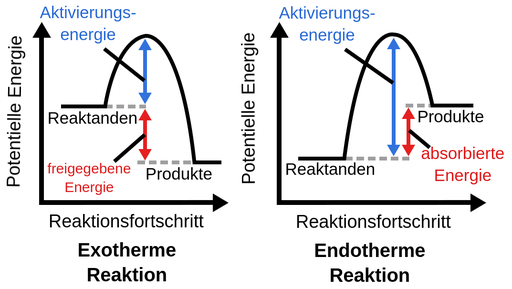
\includegraphics[width=0.9\textwidth]{endoexo}
%\caption{Verschiedene Aktivierungsenergien}


\resizebox{.9\textwidth}{!}{
\begin{tikzpicture}[
    font=\sffamily\scriptsize,
    axis/.style={-{Triangle[length=3mm, width=2.5mm]}, line width=1.2pt},
    curve/.style={line width=1.5pt},
%    dash/.style={dashed, gray, thick},
    energyarrow/.style={{Stealth[length=2.5mm]}-{Stealth[length=2.5mm]}, thick},
    pointer/.style={thick, shorten >=2pt},
]

% ==========================================
% LINKER GRAPH: Exotherme Reaktion
% ==========================================
\begin{scope}
    % Achsen
    \draw[axis] (0,0) -- (0,4.5) node[yshift=0.7cm,midway, left=0.2cm, rotate=90, font=\sffamily\small] {               Potentielle Energie};
    \draw[axis] (0,0) -- (4.5,0) node[midway, below=0.2cm, font=\sffamily\small] {Reaktionsfortschritt};
    
    % Titel
    \node[below, align=center, font=\sffamily\small\bfseries] at (2.25,-0.8) {Exotherme\\[-0.5ex]Reaktion};

    % Kurve (Start bei y=2.5, Peak bei x=2/y=4, Ende bei y=1)
    \draw[curve] (0.2, 2.5) -- (1.2, 2.5) 
                 .. controls (1.6, 2.5) and (1.6, 4) .. (2, 4) 
                 .. controls (2.4, 4) and (2.4, 1) .. (2.8, 1) 
                 -- (4.2, 1);
                 
    % Gestrichelte Hilfslinien
    \draw[dashed] (1.2, 2.5) -- (2.5, 2.5);
    \draw[dashed] (2.5, 1) -- (2.8, 1);
    
    % Beschriftung der Energieniveaus
    \node[below] at (0.7, 2.5) {Reaktanden};
    \node[below] at (3.5, 1) {Produkte};
    
    % Energie-Pfeile
    \draw[energyarrow, miugray2] (2, 2.5) -- (2, 4);
    \draw[energyarrow, petunitext] (2, 1) -- (2, 2.5);
    
    % Pointer und Text für die Pfeile
    \node[miugray2, align=center] (ea1) at (0.8, 3.8) {Aktivierungs-\\energie};
%    \draw[pointer] (ea1) -- (2.15, 3.25);
    
    \node[petunitext, align=center] (de1) at (0.8, 1) {freigegebene\\Energie};
%    \draw[pointer] (de1) -- (2.15, 1.75);
\end{scope}

% ==========================================
% RECHTER GRAPH: Endotherme Reaktion
% ==========================================
\begin{scope}[yshift=-6.5cm]
    % Achsen
    \draw[axis] (0,0) -- (0,4.5) node[yshift=0.7cm,midway, left=0.2cm, rotate=90, font=\sffamily\small] {Potentielle Energie};
    \draw[axis] (0,0) -- (4.5,0) node[midway, below=0.2cm, font=\sffamily\small] {Reaktionsfortschritt};
    
    % Titel
    \node[below, align=center, font=\sffamily\small\bfseries] at (2.25,-0.8) {Endotherme\\[-0.5ex]Reaktion};

    % Kurve (Start bei y=1, Peak bei x=2/y=4, Ende bei y=2.5)
    \draw[curve] (0.2, 1) -- (1.2, 1) 
                 .. controls (1.6, 1) and (1.6, 4) .. (2, 4) 
                 .. controls (2.4, 4) and (2.4, 2.5) .. (2.8, 2.5) 
                 -- (4.2, 2.5);
                 
    % Gestrichelte Hilfslinien
    \draw[dashed] (1.2, 1) -- (2.8, 1);
    \draw[dashed] (2.5, 2.5) -- (2.8, 2.5);
    
    % Beschriftung der Energieniveaus
    \node[below] at (0.7, 1) {Reaktanden};
    \node[right] at (2.8, 2.3) {Produkte};
    
    % Energie-Pfeile 
    \draw[energyarrow, miugray2] (2, 2.5) -- (2, 4);
    \draw[energyarrow, petunitext] (2, 1) -- (2, 2.5);
    
    % Pointer und Text für die Pfeile
    \node[miugray2, align=center] (ea2) at (0.8, 3.8) {Aktivierungs-\\energie};
%    \draw[pointer] (ea2) -- (2.45, 3.25); 
    
    \node[petunitext, align=center] (de2) at (4, 0.8) {absorbierte\\Energie};
%    \draw[pointer] (de2) -- (2.55, 1.75);
\end{scope}

\end{tikzpicture}
}
\end{marginfigure}

\textbf{Q10} ist der Faktor um den sich die Reaktionsgeschwindigkeit erhöht, wenn man die Temperatur um 10°C erhöht. \par
\textbf{Z-Wert} ist die Temperaturdifferenz, die benötigt wird um die Reaktionsgeschwindigkeit um den Faktor 10 zu erhöhen. \pp

\subsection{Effekte des Blanchierens}
\begin{itemize}
\item Inaktivierung der Enzyme
\item Elimination von Sauerstoff
\item Farbe
\item Reduktion der Keimbelastung
\item Schrumpfen bzw. Erweichen der Rohware
\item Entfernen von unerwünschten Aromastoffen
\end{itemize}
\pp

\subsection{Pasteurisation}
\marginnote[
Es wurden zwei Videos gezeigt über YouTube:\par 
Tunnelpasteur-Video KHS INNOPAS \par 
JBT Hydromatic Hydrostatic Sterilizer
]{}[0cm]
\antwort{pH 4,5 $>$ Pasteurisation \par pH 4,5 $<$ Sterilisation }


\subsection{Abtöten von Mikroorganismen}



Kinetik erster Ordnung:
\begin{align*}
\frac{dN}{dt} = - k \cdot N
\end{align*}
Wobei $k$ die Reaktionsgeschwindigkeit in 1/s darstellt. \par 
Für die Zahl der Mikroorganismen $N$ nach einer Zeit $t$ lässt sich folgende Formel aufstellen:
\begin{align*}
N(t) = N_0 \cdot e^{-k \cdot t}
\end{align*}


\begin{figure}[h]

\begin{center}
\begin{tikzpicture}
\node[anchor=west] at (0,0){
\begin{tikzpicture}
\draw[->] (0,0) to (0,4) node[right] {$N$};
\draw[->] (0,0) to (4,0) node[right] {$t$};
\draw[-,miugray2] (0,3.5) to (3.5,0);
\draw (-0.1,3.5) node[left] {$10^6$} to (0,3.5);
\draw (-0.1,2.5) node[left] {$10^5$} to (0,2.5);
\draw (-0.1,1.5) node[left] {$10^4$} to (0,1.5);
\draw (-0.1,0.5) node[left] {$10^3$} to (0,0.5);
\draw (0,-0.1) node[below,scale=0.7] {1 min} to (0,0);
\draw (1,-0.1) node[below,scale=0.7] {2 min} to (1,0);
\draw (2,-0.1) node[below,scale=0.7] {3 min} to (2,0);
\draw (3,-0.1) node[below,scale=0.7] {4 min} to (3,0);
\draw [dashed,petunitext] (1,2.5) to (1,1.5);
\draw [<->, petunitext] (1,1.5) to node[below,scale=1,yshift=-2mm] {$D_t$}(2,1.5);
\end{tikzpicture} };
\node[anchor=west] at (6,0){
\begin{tikzpicture}
\draw[->] (0,0) to (0,4) node[right] {$D$ (min)};
\draw[->] (0,0) to (4,0) node[right] {$T$ (°C)};
\draw[-,miugray2] (0,3.5) to (3.5,0);
\draw (-0.1,3.5) node[left] {100} to (0,3.5);
\draw (-0.1,2.5) node[left] {10} to (0,2.5);
\draw (-0.1,1.5) node[left] {1} to (0,1.5);
\draw (-0.1,0.5) node[left] {0.1} to (0,0.5);
\draw (0,-0.1) node[below,scale=0.7] {60} to (0,0);
\draw (1,-0.1) node[below,scale=0.7] {70} to (1,0);
\draw (2,-0.1) node[below,scale=0.7] {80} to (2,0);
\draw (3,-0.1) node[below,scale=0.7] {90} to (3,0);
\draw [dashed,petunitext] (1,2.5) to (1,1.5);
\draw [<->, petunitext] (1,1.5) to node[below,scale=1,yshift=-2mm] {Z}(2,1.5);
\end{tikzpicture} };
\end{tikzpicture}
\caption{Linker Graph - Mikroorganismen über Zeit ; Rechter Graph D-Wert über Temperatur}
\end{center}

\end{figure}

\pp
Der \textbf{D-Wert} ist die Zeit, die man erhitzen muss, um die Keimzahl auf ein Zehntel zu reduzieren. \par 
Der \textbf{Z-Wert} ist die erforderliche Temperaturerhöhung, die nötig ist, um den D-Wert um eine Zehnerpotenz zu reduzieren
\pp

\awesomebox[petunitext]{1mm}{\faExclamationTriangle}{miugray2}{\textbf{12D-Konzept:} \textit{Clostridium botulinum} muss 12 mal um ein Zehntel reduziert werden, damit es als abgestorben gilt. \textit{Clostridium botulinum} dient als Leitkeim für sichere Konserven nach dem 12D-Konzept}
\begin{figure}
\centering
\resizebox{.4\textwidth}{!}{
\begin{tikzpicture}
\draw[->] (0,0) to (0,4) node[right] {$N$};
\draw[->] (0,0) to (8,0) node[right] {$t$};
\draw[rounded corners=4pt] (0,3.5) .. controls (0.5,2) and (0.9,1) .. (2.5,0.5) .. controls (3.5,0.4) .. (5.5,0.3) to (8,0.2);
\end{tikzpicture}
}
\caption{Verlaufskurve Abtöten von Mikroorganismen}
\end{figure}

\pagebreak
\section*{Vorlesung 12 - Haltbarmachung}\addtocounter{section}{1}

\subsection{D-Wert}
Wie bereits in der letzten Vorlesung erwähnt, ist der \textbf{D-Wert} die Zeit, die man erhitzen muss, um die Keimzahl auf ein Zehntel zu reduzieren. Um den D-Wert für eine bestimmte Temperatur zu errechnen, können wir uns folgende Formel herleiten:

\begin{align*}
z &= \frac{T_2 - T_1}{\log(D_1) - \log(D_2)} \\
 &= \frac{T_2 - T_1}{\log(\frac{D_1}{D_2})} \\
\log(\frac{D_1}{D_2}) &= \frac{T_2 - T_1}{z} \\
\frac{D_1}{D_2} &= 10^{\frac{T_2 - T_1}{z}} \\
D_1 &= D_2 \cdot 10^{\frac{T_2 - T_1}{z}} 
\end{align*}

\antwort{\begin{align}
D_1 &= D_2 \cdot 10^{\frac{T_2 - T_1}{z}} 
\end{align}
}



%\reversemarginpar
\subsection{F-Wert}
Der \textbf{F-Wert} ist definiert als die Summe aller letalen Effekte, die im Verlauf einer Erhitzung auf eine Mikroorganismen-Population wirken. Der F-Wert beschreibt den Erhitzungseffekt, also die Keimabtötungsrate. Dabei geht man von folgendem Grundwert aus:

\pp
\begin{center}
1 F-Wert = 1 Minute bei 121°C
\end{center}

\pp
Zur Berechnung des jeweiligen F-Wertes nutzen wir folgende Formel:
\antwort{
\begin{align}
F = D(\log N_0 - \log N(t) )
\end{align}}

\subsubsection{Beispielberechnung}
Vor der Sterilisation beträgt die Keimzahl 1 Spore \textit{Clostridium botulinum} pro Gramm Lebensmittel. Da \textit{Clostridium botulinum} ein gefährlicher Toxinbildner ist, wird das sogenannte 12-D-Konzept angewendet, um auf 10$^{-12}$ Sporen pro Gramm Lebensmittel zu reduzieren, um eine ausreichende Sicherheit zu gewährleisten.\par 
Im Ergebnis enthält dann jedes billionste Gramm des Lebensmittels noch eine überlebende Spore, oder bei 1000 g-Dosen noch jede milliardenste Dose. Aus diesen Werten für den Leitkeim \textit{Clostridium botulinum} (D-Wert: 0,2 min) und den Anforderungen ergibt sich:
\begin{align*}
F &= 0,2 ~\text{min} \cdot (\log (1) - \log (10^{-12})) = 2,4 ~\text{min}
\end{align*}
Daher müssen wir 2,4 min bei 121°C erhitzen um eine ausreichende Sicherheit des Lebensmittels zu gewährleisten.

\subsubsection{Letalitätswert}

\marginnote[Je kleiner der Letalitätswert, desto effektiver \pp L = 1 \RA 121°C bei 1min \par L = 0,1 \RA 121°C bei 0,1min]{}[0pt]
Der \textbf{Letalitätswert} $L$, auch Letalitätsrate oder Teil-F-Wert (F abgeleitet von Fahrenheit) genannt, gibt an, wie effektiv Mikroorganismen mit definierter Hitzeresistenz abgetötet werden, wenn sie eine Minute lang einer bestimmten Temperatur ausgesetzt werden. \pp
In der Berechnung des konkreten Letalitätswertes bei der Untersuchung einer Probe spielen die Dezimale Reduktionszeit und der Z-Wert eine Rolle. \pp
So lässt sich der L-Wert wie folgt berechnen:


\begin{align*}
L = \frac{F_0}{F_t} = \frac{D(121,1)}{D_t} = 10^{\frac{T-121,1}{z}}
\end{align*}


\subsubsection{Erhitzungsprozess}
\marginnote[L-Wert gilt für idealen Erhitzungsprozess]{}[0pt]
\begin{figure}[h]
\centering
\begin{tikzpicture}
\draw[->] (0,0) to (0,4) node[right] {$T$};
\draw[->] (0,0) to (8.5,0) node[right] {$t$};

\draw[petunitext] (0,0) .. controls (2.5,4) and (5.5,4)  .. (8,0) node[above,yshift=15mm,xshift=-6mm] {real};
\draw[miugray2] (2.5,0) to (2.5,3) node[below,xshift=15mm] {ideal} to (5.5,3) to (5.5,0);
\end{tikzpicture}
\caption{Realer vs. Idealer Erhitzungsprozess}
\end{figure}

\newpage
% ==========================================
% VORLESUNG 13 + 14
% ==========================================
%%%\sidebar
%\miushead{Vorlesung 13 + 14 - PLMT}{Vorlesung 13 + 14}
%\par \vspace*{5mm}
\section*{Vorlesung 13 - Verdampfen}
\addtocounter{section}{1}
\subsection{Phasendiagramm}
Um Wasser aus der flüssigen Phase in die gasförmige Phase zu überführen, können wir dies durch eine \textbf{Temperaturerhöhung} oder \textbf{Druckerniedrigung} realisieren.

\begin{figure}[h]
\centering
\begin{tikzpicture}[scale=0.8]
\draw[->] (0,0) to (4,0) node[right] {$T$};
\draw[->] (0,0) to (0,4) node[right] {$p$};
\draw[-, rounded corners=5pt] (0.5,0.5) to (1,1) to (1,3);
\draw[-, petunitext] (1,1) to [bend right=35](3,3);
%\draw[<->, miugray2!60,dashed] (0.5,2) to (3.5,2);
%\draw[<->, miugray2!60,dashed] (1.5,2.5) to (1.5,0.5);
\node[scale=0.7] at(1.75,2.5) {\large \bfseries flüssig};
\node[scale=0.7] at(3,1) {\large \bfseries gasförmig};
\node[scale=0.7,rotate=90] at(0.5,2) {\large \bfseries fest};
\end{tikzpicture}
\caption{Dampfdruckkurve}
\label{Dampfdruckkurve}
\end{figure}

Ähnlich wie in Abbildung \ref{Dampfdruckkurve} können wir in Abbildung \ref{Saccharose} sehen, dass auch eine Sättigungslinie einer Saccharose-Lösung sich ähnlich wie eine Dampfdruckkurve verhält. Es wird ein Gleichgewichtszustand beschrieben der sich mathematisch in Abhängigkeit von Druck und Temperatur bestimmen lässt.
%\footnotesize
%\textit{Ein Phasendiagramm (auch Zustandsdiagramm, Zustandsschaubild oder Gleichgewichtsschaubild) ist eine Projektion von Phasengrenzlinien aus dem Zustandsraum eines thermodynamischen Systems in ein zweidimensionales kartesisches Koordinatensystem. Verschiedene Zustände lassen sich über die Clausius-Clapeyron-Gleichung berechnen.}
%\normalsize

\begin{marginfigure}[-8cm]
\resizebox{\textwidth}{!}{
\begin{tikzpicture}[x=1.2cm, y=1.2cm, font=\sffamily]

    % Define colors sampled from the uploaded image
    \definecolor{colorLabil}{RGB}{90, 117, 147}
    \definecolor{colorInter}{RGB}{149, 178, 206}
    \definecolor{colorMeta}{RGB}{197, 215, 232}
    \definecolor{colorUnsat}{RGB}{230, 238, 245}

    \def\xmax{7}
    \def\ymax{6}

    % 1. Fill entire area with ungesättigter background
    \fill[miugray2!7] (0,0) rectangle (\xmax,\ymax);

    % 2. Fill metastabil area (and everything above it)
    \fill[miugray2!20] (0,\ymax) -- (0,0.8) .. controls (4,1.2) and (5.5,3.0) .. (6.5,\ymax) -- cycle;

    % 3. Fill intermediär area (and everything above it)
    \fill[miugray2!30] (0,\ymax) -- (0,1.6) .. controls (3.5,2.0) and (4.8,3.5) .. (5.5,\ymax) -- cycle;

    % 4. Fill labil area
    \fill[miugray2!60] (0,\ymax) -- (0,2.5) .. controls (2.5,2.8) and (3.8,4.0) .. (4.5,\ymax) -- cycle;

    % Draw the separation curves
    \draw[thick] (0,0.8) .. controls (4,1.2) and (5.5,3.0) .. (6.5,\ymax);
    \draw[thick] (0,1.6) .. controls (3.5,2.0) and (4.8,3.5) .. (5.5,\ymax);
    \draw[thick] (0,2.5) .. controls (2.5,2.8) and (3.8,4.0) .. (4.5,\ymax);

    % Draw the axes
    \draw[->, very thick] (0,0) -- (\xmax+0.5,0) node[below left=2pt] {\Large Temperatur};
    \draw[->, very thick] (0,0) -- (0,\ymax+0.5) node[above left=2pt, rotate=90] {\Large Anteil Zucker};

    % Add region labels
    \node[rotate=0] at (1.1, 4) {\Large \textbf{labil}};
    \node[rotate=0] at (1.2, 2.4) {\textbf{intermediär}};
    \node[rotate=0] at (1.2, 1.5) {\textbf{metastabil}};

    \node[align=center] at (5.0, 1.2) {\Large \textbf{ungesättigter}\\[1ex] \Large \textbf{Bereich}};
    
    \draw[->, very thick,red] (4,0.2) -- (2,0.2) node[above] {Abkühlung};
    \draw[->, very thick,red] (6.8,2.5) -- (6.8,5) node[left,rotate=90,yshift=3mm,xshift=-1mm] {Verdampfung};
    \draw[->, very thick,red] (5,2.5) -- (2,5) node[midway, rotate=-40,yshift=4mm] {\large Flash Evaporation};

\end{tikzpicture}
}
\caption{Schematische Darstellung des Zusammenhangs von Temperatur und Verdampfung auf die Kristallbildung in einer Saccharoselösung.}
\label{Saccharose}
\end{marginfigure}

\subsection{Energie für Verdampfung berechnen}

Für die Verdampfung benötigte Wärmezufuhr $\dot{Q}_H$:
\pp
\antwort{
\begin{align}
\dot{Q}_H = \dot{m}_D \cdot \Delta h_v + \dot{m}_F \cdot c_{p,F} \cdot (T_S - T_F)
\end{align}
\vspace*{-2mm}
}
\reversemarginpar
\marginnote[Der Begriff \textbf{Brüden} bezeichnet in der Regel mit Wasserdampf gesättigte Luft, die beim Trocknen von Feststoffen entsteht.]{}[1cm]
\pp
Wobei: \par
\begin{multicols}{2}
$\dot{m}_D$ = Massenstrom des Brüden \par
$\dot{m}_F$ = Massenstrom des Zulaufs (F \RA feed) \par 
$T_S$ = Siedetemperatur \par 
$T_F$ = Temperatur des Zulaufs \par
\end{multicols}

\subsection{Sattdampf}
\begin{itemize}
\item $T$, $p$ durch Dampfdruckkurve definiert
\item keine Nebeltröpfchen
\item Wärmeentzug \RA Bildung von Nebeltröpfchen durch Kondensation \RA \textbf{Nassdampf}
\item Wenn Wärmeentzug sehr vorsichtig vollzogen wird \RA \textbf{übersättigter Dampf}
\item Bei erhitzen \RA \textbf{Überhitzter Dampf} (Brüden)
\end{itemize}

\pagebreak
\subsection{Dampfdruckkurve}
Beschreibung der Dampfdruckkurve durch die Beziehung von \textbf{Clausius-Clapeyron}:
\begin{align*}
\ln \frac{p_2}{p_1} = \frac{\Delta h_v M_L}{R} \cdot ( \frac{1}{T_1} - \frac{1}{T_2} )
\end{align*}

Wobei: \par
\begin{multicols}{2}
$p$ = Dampfdruck \par 
$R$ = Universelle Gaskonstante \par 
$\Delta h_v$ = mittlere spezifische Verdampfungsenthalpie \par 
$M_L$ = molare Masse des Lösungsmittels \par 
$\Delta h_{vM}$ = mittlere molspezifische Verdampfungsenthalpie
\end{multicols}
\pp
Nach Umformen erhalten wir
\begin{align*}
\Delta h_{vM} = \frac{R \cdot T_1 \cdot T_2 \cdot \ln(\frac{p_2}{p_1})}{T_2 - T_1}
\end{align*}

Die oben stehende Formel lässt sich unter der Annahme, dass ein ideales Gas vorliegt und das Molvolumen eines Gases größer als das einer Flüssigkeit ist, vereinfachen und es gilt annäherungsweise\par 
\antwort{

\begin{align}
\Delta h_{vM} = \frac{R \cdot T^2}{\Delta T} \cdot \frac{\Delta p}{p_0}
\end{align}
\color{miudiutex}
}


\subsection{Siedepunkterhöhung}
\subsubsection{Durch gelösten Stoff} 
\textit{Beispiel: Salz in Nudelwasser} \par 
Wir können eine Siedepunkterhöhung durch das Lösen eines Stoffes (mit vernachlässigbarem kleinem Dampfdruck) erreichen. \par Die Dampfdruckerniedrigung $\Delta p$ ist proportional zu dem Stoffmengenanteil $x_i$ des gelösten Stoffes $i$
\reversemarginpar
\marginnote[\small Raoultsches Gesetz zur Berechnung des Gas-Flüssig-Gleichgewichts \RA]{}[1cm]
\pp
\antwort{


\begin{align}
\Delta p = x_i \cdot p
\end{align} 
}
\par \vspace*{2mm}
\color{miudiutex}

Der Stoffmengenanteil $x_i$ berechnet sich aus dem Verhältnis von unserem Stoff $i$ im Verhältnis zur Gesamten Stoffmenge:
\begin{align*}
x_i = \frac{n_i}{n_{tot}}
\end{align*}


Für Salze gilt:
\begin{align*}
n_i = n_{Salz} \cdot [1+ \delta \cdot (z-1)]
\end{align*}
Wobei: \par 
$\delta$ = Dissoziationsgrad des Salzes \par 
$z$ = Anzahl Ionen pro Formeleinheit des Salzes \pp

\pagebreak
Formel zur Berechnung der Temperaturdifferenz des Siedepunkts bei Zugabe eines Lösungsmittels:

\begin{align*}
\Delta T &= \frac{R \cdot T^2}{\Delta h_{vM}} \cdot \frac{\Delta p}{p_0} \\
\Delta T &= \frac{R \cdot T^2}{\Delta h_{vM}} \cdot x_i \\
&\approx \frac{R \cdot T^2}{\delta_L \cdot \Delta h_v} \cdot c_i
\end{align*}
\antwort{

\begin{align}
\Delta T &\approx \frac{R \cdot T^2}{\delta_L \cdot \Delta h_v} \cdot c_i
\end{align}
\color{miudiutex}
}
\pp
Wobei:\par 
$\delta_L$ = Dichte des Lösungsmittels \par 
$c_i$ = molare Konzentration des gelösten Stoffes i [mol/m$^3$]

 


\subsubsection{Durch hydrostatischen Druck}
\textit{Beispiel: Kochen im Vakuum oder Druckkessel}
\begin{align*}
\Delta T = \frac{R \cdot T^2}{\Delta h_{vM}} \cdot \frac{\rho_{lg} \cdot g \cdot h}{p}
\end{align*}
Wobei: \par
$\rho_{lg}$ = Dichte der Flüssigkeits-Dampf-Säule mit Dampfanteil $\varepsilon$
\begin{align*}
\rho_{lg} = (1 - \varepsilon) \cdot \rho_l
\end{align*}
$\rho_l$ = Dichte der Flüssigkeit ist


\subsection{Beispielvideos}
Thin Film Evaporation Process \par 
LCI Corporation \pp
Pfaudler Wiped Film Evaporator (WFE) - Construction and Operation \par 
GMM Pfaudler \pp
Falling Film Evaporator \par 
gea.com \pp

\subsection{Brüdenverdichtung}
\begin{marginfigure}[-3.5cm]
%\centering
\resizebox{1\textwidth}{!}{
\begin{tikzpicture}
\draw (0,0) to (0,1);
\draw (-1,0.8) to (0,0.8);
\draw (0,3) to (0,1.5) to (0.25,1) to (0.25,0.8);
\draw[xscale=-1,xshift=-1cm] (0,3) to (0,1.5) to (0.25,1)to (0.25,0.8);
\draw (1,0) to (1,1);
\draw[->,miugray2] (0.5,2.5) to (0.5,1.5) node[right,xshift=2mm,yshift=1mm,rotate=90] {\footnotesize $T_1$, $p_1$};
\draw[->,petunitext] (-1,1.1) to (-0.6,1.1) node[above,xshift=-3mm,scale=0.8,yshift=1mm] {Brüden};
\draw[dashed,rounded corners=5pt,->,petunitext!65] (-0.5,1.1) to (0.1,1.1) to (0.25,0.3);
\draw (-1,1.6) to (0,1.6);
\end{tikzpicture}
}
\caption{Brüden\-verdichtung}
\label{fig1}
\end{marginfigure}

In \textbf{Abbildung \ref{fig1}} wird gezeigt, wie durch eine Verengung eines Rohres Wasserdampf fließt und ein Unterdruck entsteht. Der Brüden der von der Seite hinzuströmt wird ''eingesogen'' und durch diese Kraft verdichtet.\par
Durch die Verdichtung des Brüden lässt sich ein hoher Teil der Energie, die ursprünglich zum Erhitzen des Lebensmittels aufgewendet wurde, zurückgewinnen. Eine Folie aus der Vorlesung zeigt den Mechanismus der Energierückgewinnung in einem Mehrstufenprinzip.


\pagebreak

\section*{Vorlesung 14 - Trocknen}\addtocounter{section}{1}
\subsection{Welche Lebensmittel trocknen wir?}
An der Tafel wurden sämtliche Ideen der Studenten gesammelt: \par 
Chips, Obst, Gemüse, Gewürze, Fleisch, Fisch, Kaffee, Tee, Kakao, Backwaren, Teigwaren, Milch, Getreide, Algen, Hülsenfrüchte, etc.
\pp
\antwort{
Das Trocknen bzw. die Haltbarmachung durch Wasserentzug ist eines der ältesten Haltbarmachungsmethoden der Menschheit. Welche Gründe des Trocknens kennen wir noch?
}

\subsection{Effekte des Trocknens}
\subsubsection{Erwünschte Effekte}
\begin{itemize}
\item Konservierung, Haltbarmachung
\item Reduktion von Gewicht und Volumen
\item Änderung der Struktur und technofunktionellen Eigenschafte
\end{itemize}

\subsubsection{Unerwünschte Effekte}
\begin{itemize}
\item Verlust bzw. Veränderung von wertgebenden Inhaltsstoffen / Eigenschaften
\begin{itemize}
\item Vitamine
\item Textur
\item Aroma
\item Farbe
\item Volumen, Form
\end{itemize}
\end{itemize}

\subsection{Abtrennen von Wasser}

\begin{multicols}{2}

\subsubsection{Aus feuchter Luft}
\begin{itemize}
\item Adsorption (zum Beispiel wenn ein Lebensmittel Wasser aus der Luft aufnimmt)
\item Kondensation (Spiegel im Badezimmer)
\item Bildung von Kristallwasser (CaCl$_2$)
\end{itemize}

\columnbreak
\subsubsection{Aus wasserhaltigen Flüssigkeiten}
\begin{itemize}
\item Verdampfen (Destillation)
\item Zentrifugieren
\item Bildung von Kristallwasser
\end{itemize}
\end{multicols}

\subsubsection{Mechanische Verfahren}
\begin{itemize}
\item thermische Verfahren \RA Verdampfung oder Sublimationen
\end{itemize}

\subsection{Beispiel}
Wir wollen einen Apfelring trocknen. Wie gehen wir vor?

\begin{marginfigure}[-8cm]
\centering
\resizebox{.9\textwidth}{!}{
\begin{tikzpicture}[node distance=1.5cm]
\node (waermezufuhr) {Wärmezufuhr};
\node (temperaturerhoehung) [below of=waermezufuhr] {Temperaturerhöhung};
\node (dampfdruckerhoehung) [below of=temperaturerhoehung] {Dampfdruckerhöhung};
\node (verdampfung) [below of=dampfdruckerhoehung] {Verdampfung};
\node (temperaturabsenkung) [below of=verdampfung] {Temperaturabsenkung};

\draw[->] (waermezufuhr) -- (temperaturerhoehung);
\draw[->] (temperaturerhoehung) -- (dampfdruckerhoehung);
\draw[->] (dampfdruckerhoehung) -- (verdampfung);
\draw[->] (verdampfung) -- (temperaturabsenkung);

\node (1) [below of=temperaturabsenkung,petunitext, align=center, scale=0.7,yshift=1.5cm] {\RA begünstigt \\ Wärmetransport};
\end{tikzpicture}
}
\caption{Trocknungsprozess}
\end{marginfigure}

Der Erfolg unseres Trockungsprozesses des Apfelrings hängt vorallendingen von Faktoren wie dem Verhältnis zur Oberfläche (zum Volumen), Temperatur, Druck, relative Feuchte und der Zusammensetzung des Produktes ab.

\newpage
% ==========================================
% VORLESUNG 15 + 16
% ==========================================
%%%\sidebar
%\miushead{Vorlesung 15 + 16 - PLMT}{Vorlesung 15 + 16}
%\par \vspace*{5mm}
\section*{Vorlesung 15 - Trocknen}\addtocounter{section}{1}
\subsection{Trocknungsverlauf bei Konvektionstrocknung}

\begin{figure}[h]
\centering
\begin{tikzpicture}
\draw[->] (0,0) to (0,4) node[right,align=left] {Trocknungs- \\ geschwindigkeit};
\draw[->] (0,0) to (6,0) node[right] {Wassergehalt};

\draw (0,1) .. controls (1.5,1) and (2.5,1) .. (4,3) to (6,3);
\node[petunitext,scale=1.2](1)at(5,3.5){\bfseries\sffamily Phase I};
\node[petunitext,scale=1.2](2)at(1.5,2){\bfseries\sffamily Phase II};

\node[miugray2!50!miudiutex,align=center,scale=0.8] (3) at (5,1) {Gleichgewichtsfeuchte \\ hygroskopischer LM};
\draw[miugray2,dashed, <-, shorten <= 5pt] (0.5,1) to [bend right=25] (3.west);
\end{tikzpicture}
\caption{Verschiedene Phasen des Trocknungsprozesses}
\end{figure}
\begin{multicols}{2}
\subsubsection*{Phase I}
\begin{itemize}
\item konstante Trocknungsgeschwindigkeit
\item dünner Flüssigkeitsfilm an der Oberfläche
\item konstante Temperatur (Kühlgrenztemperatur)
\end{itemize}
\columnbreak
\subsubsection*{Phase II}
\begin{itemize}
\item Oberfläche ist ausgetrocknet
\item Trockenspiegel verschiebt sich in das LM
\item sinkende Trocknungsgeschwindigkeit
\item Temperatur der Oberfläche steigt an
\end{itemize}
\end{multicols}
\ppbig
\begin{figure}[h]
\centering
\begin{tikzpicture}[scale=0.9]
\draw[->] (0,0) to (0,4) node[right,align=left] {Wassergehalt};
\draw[->] (0,0) to (6,0) node[right] {Zeit};

\draw[rounded corners=5pt] (0,3) .. controls (1,2.75) .. (1.9,2.1) .. controls (3,1.25) .. (5,1) to (6,1);
\draw[dashed] (2,2) to [bend right=15] (4,0);

\node(a)at(5,1.5){hygroskopische LM};
\node[align=center,scale=0.8](b)at(1.7,0.6){nicht \\ hygroskopische LM};

\end{tikzpicture}
\caption{Trocknung von hygroskopischen und nicht-hygroskopischen Lebensmitteln}
\end{figure}

\antwort{
Konvektionstrocknung kann ähnlich wie das Kühlen des Brüden beim Verdampfen mit \textbf{Gleichstrom} oder \textbf{Gegenstrom} erfolgen!
}

\pagebreak
%\setcounter{section}{2}
\section*{Vorlesung 16 - Gefrieren}\addtocounter{section}{1}

\subsection{Kristallkeimbildung}
\subsubsection*{Latente Wärme}
Einsetzende Kristallbildung erzeugt Wärme, da die Kristallbildung Energie erfordert

\begin{figure}[h]
\centering
\begin{tikzpicture}
\draw (0,0) to (8,0) node[right] {Zeit};
\draw (0,0) to (0,4.5) node[right] {Temperatur};

\draw[dashed,gray] (0,0.5) node[left] {$\sigma_f$} to (8,0.5);
\draw[dashed,gray] (0,2.5) node[left] {$\sigma_a$} to (8,2.5);
\draw (0.5,3.5) to (2.5,2) to (3,2.5) to (6,1.5) to (6.5,1.75) to (7,1.50) to (8,0.5);
\draw[<->] (2.5,2.5) to node [left,scale=0.7,xshift=-5mm] {Latente Wärme} (2.5,2);
\end{tikzpicture}

\end{figure}

\ppbig
\begin{multicols}{2}
\subsubsection*{Geringe Gefriergeschwindigkeit}
\begin{itemize}
\item Bildung der Eiskristalle zunächst an Orten mit geringerer Konzentration gelöster Stoffe (v.a. Zellzwischenräume)
\item Austritt von Wasser aus den Zellen in Zellzwischenräume
\item Entstehung großer unförmiger Eiskristalle
\item Deformation der Zellen
\end{itemize}

\columnbreak
\subsubsection*{Hohe Gefriergeschwindigkeit}
\begin{itemize}
\item Eisbildung im intra- und extrazellulärem Raum
\item Entstehung vieler kleiner Eiskristalle
\item keine Zelldeformation
\item Konsistenz bleibt beim Auftauen erhalten
\item v.a. Bereich der Kristallkeimbildung sollte schnell durchlaufen werden (0 bis 5°C)
\end{itemize}
\end{multicols}

\pagebreak

\section*{Vorlesung 17 - Verderb}\addtocounter{section}{1}
\antwort{
\textbf{MHD} ist das Datum, bis zu dem das Lebensmittel, bei richtiger Aufbewahrung, seine spezifischen Eigenschaften behält. \pp
\textbf{Verbrauchsdatum} ist das Datum, ab dem das Lebensmittel als nicht mehr sicher gilt.\pp
\textit{VO (EU) Nr. 1169/2011}
}
\subsection{Arten von Verderb und deren Einteilung}
%\begin{multicols}{2}
Wir können Verderb in 3 Kategorien einteilen: in eine Änderung von sensorischen Eigenschaften, der Sicherheit oder auch Änderung von Inhaltsstoffen.
\pp
\subsubsection{Woran erkennt man Verderb?}
\begin{itemize}
\item \textbf{Geruch} (Fäulnis, Gärungsgerüche, Ranzigkeit)
\item \textbf{Aussehen} (Farbe, Trübungen, Optische Veränderung durch Phasentrennung)
\item \textbf{Textur} (weichwerden oder auch austrocknen; schleimig, schmierig, Gasbildung)
\item \textbf{Geschmack} (Säuerung, Entstehung von Bitterpeptiden, Selten: Süße)
\item Änderung der \textbf{Inhaltsstoffe} (Infektions- und Intoxikationsrisiko)
\begin{itemize}
\item Toxine (Mykotoxine, Botulinum-Toxin, Ethanol, Staphylokokken-Endotoxine, etc.)
\item Verlust von Vitaminen, Fettsäuren, Aminosäuren, Farb-, Aroma- und Geschmacksstoffe
\item Bakterien (z.B.: Salmonellen, Listerien, Campylobacter)
\item Viren (Norovirus)
\end{itemize}
\end{itemize}

%\columnbreak
\subsubsection{Welche Prozesse liegen dem zugrunde?}
\begin{itemize}
\item \textbf{Mikrobieller Verderb}
\item \textbf{Chemischer Verderb}
\begin{itemize}
\item Oxidation
\item Hydrolyse
\item Unerwünschte Maillard-Reaktion
\end{itemize}
\item \textbf{Physikalischer Verderb}
\begin{itemize}
\item Austrocknen, Entnahme von Wasser
\item Quellung, Aufnahme von Wasser
\item Kristallisation
\item Trennung von Emulsionen
\end{itemize}
\item \textbf{Enzymatischer Verderb}
\begin{itemize}
\item Enzymatische Bräunung (Polyphenoloxidasen)
\item Hydrolyse von Lipiden, Kohlenhydraten und Eiweißen
\item Gewebserweichung durch Pektinesterasen
\item Lipoxigenasen (führen bsp. zu fischigen Aromen bei Muttermilch wenn man sie nicht ausreichend erhitzt - selbst bei Lagerung im Tiefkühl)
\end{itemize}
\item \textbf{Sonstige Kontamination}, Schädlingsbefall
\end{itemize}
%\end{multicols}
\subsection{Ergänzung Folien}
\folie{Hydrolytische Veränderung}
Welche der Enzyme sind Hydrolasen? \pp
Amylasen, Pektinasen, Lipasen, Proteasen (sind aber nicht auf der Folie mit dabei)
\pp
\pp\textbf{Beispiel hydrolytische Veränderung (nicht wichtig):} \par
Freisetzung von hydroxylierten C13-Norisoprenoiden aus Carotinoiden z.B.: Grashüpfer-Keton, $\beta$-Ionon

\subsection{Säurekonstante und pKs-Wert}

\antwort{Die \textbf{Säurekonstante $\mathbf{K_S}$}
\begin{align}
K_S = \frac{[H_3O^+]\cdot [A]}{[HA]}
\end{align}
\textbf{pK$_\mathbf{S}$-Wert}
\begin{align}
pK_S = - \log_{10} \cdot K_S
\end{align}}

\pagebreak
\enlargethispage{\baselineskip}
\section*{Vorlesung 18 - Sinkgeschwindigkeit nach Stokes}\addtocounter{section}{1}

%\subsection*{Grundlagen}
\textbf{Zur Erinnerung:} Für ein kugelförmiges Teilchen im Fluid gelten folgende geometrische Beziehungen für das Volumen $V_{\text{Kugel}}$ und die Fläche $A$:
\begin{align*}
    V_{\text{Kugel}} \qquad &= \frac{4}{3}\pi r^3 \qquad = \frac{1}{6}\pi d^3 \\
    A \qquad &= \pi r^2 \qquad ~~  = \frac{1}{4}\pi d^2
\end{align*}

\subsection*{Wirksame Kräfte}
\begin{marginfigure}
\centering
\resizebox{.9\textwidth}{!}{
\begin{tikzpicture}[scale=1.6, >=stealth]
    % Wellenlinien links und rechts (Fluid-Andeutung)
%    \draw[domain=-1:1, smooth, variable=\y, shift={(-1.2,0)}] plot ({0.1*sin(\y*400)}, \y);
%    \draw[domain=-1:1, smooth, variable=\y, shift={(1.2,0)}] plot ({0.1*sin(\y*400)}, \y);
    \draw[fill=uniblau!10,draw=miugray!30] (-1.2,1.65) rectangle (1.2,-1.65);
    % Kugel
    \draw[fill=miugray!80, draw=black, thick] (0,0) circle (0.5cm);
    \node[scale=0.5] at (0.1,-0.25) {$m_T, \rho_T$};
    
    % Kraftpfeile nach oben
    \draw[->, thick] (0, 0.5) -- (0, 1.1) node[above] {$F_W$};
    \draw[->, thick] (0.3, 0.4) -- (0.3, 0.8) node[above] {$F_A$};
    \draw[->, thick] (-0.3, 0.4) -- (-0.3, 0.8) node[above] {$F_P$};
    
    % Kraftpfeil nach unten
    \draw[->, thick] (0, -0.5) -- (0, -1.1) node[below] {$F_G$};
    
    % Sinkgeschwindigkeit Pfeil
    \draw[->, dashed, black, thick] (0.3, -0.4) -- (0.3, -0.8) node[right] {$v_{\text{sink}}$};
    
	%Durchmesser Kugel Pfeil
	 \draw[<->, dotted, black, thick,rotate=35]   (-0.5,0) -- (0.5,0) node[midway,yshift=2.5mm,xshift=-1mm,scale=0.8]{$d$};
    
    % Fluid Parameter
    \node[left] at (-0.3, -0.75) {$\eta_F, \rho_F$};
\end{tikzpicture}
}
\caption{Schematische Darstellung eines kugelförmigen Teilchen in einem Fluid. \textit{Hinweis:} Bei kleinen Teilchen mit einem Durchmesser $d < 1\,\text{mm}$ kann die Trägheitskraft $F_P$ für den stationären Zustand vernachlässigt werden ($d v/dt \approx 0$).}
\end{marginfigure}

    \textbf{Gewichtskraft $F_G$:} Über die Masse des Teilchens $m_T$ und dessen Dichte $\rho_T$:
    \begin{equation}
        F_G = m_T \cdot g = \frac{\pi}{6} \cdot d^3 \cdot \rho_T \cdot g
    \end{equation}
    \textbf{Auftriebskraft $F_A$:} Entspricht der Gewichtskraft des verdrängten Fluidvolumens (Fluiddichte $\rho_F$):
    \begin{equation}
        F_A = m_F \cdot g = \frac{\pi}{6} \cdot d^3 \cdot \rho_F \cdot g
    \end{equation}
   \textbf{Widerstandskraft $F_W$:} Abhängig vom Strömungswiderstandsbeiwert $c_W$ und der Sinkgeschwindigkeit $v$:
    \begin{equation}
        F_W = c_W \cdot \frac{\rho_F}{2} \cdot v^2 \cdot A = c_W \cdot \frac{\rho_F}{2} \cdot v^2 \cdot \frac{\pi}{4} d^2
    \end{equation}
\textbf{Trägheitskraft $F_P$:} Beschleunigungskraft inklusive der hydrodynamisch ''mitbewegten'' Fluidmasse:
    \begin{equation}
        F_P = \left(m_T + \frac{m_F}{2}\right) \cdot \frac{dv}{dt} = \frac{\pi}{6} \cdot d^3 \cdot \left(\rho_T + \frac{\rho_F}{2}\right) \cdot \frac{dv}{dt}
    \end{equation}
    
    




%\pagebreak


%\subsection*{Welche Kräfte wirken auf das Teilchen ein?}
%Im stationären Zustand (konstante Sinkgeschwindigkeit, $F_P = 0$) hält die Gewichtskraft den entgegengesetzten Kräften (Auftrieb und Widerstand) das Gleichgewicht:
%\begin{equation}
%    F_G = F_A + F_W
%\end{equation}
%\begin{figure}[h]
%\centering
%\begin{tikzpicture}[scale=1.6, >=stealth]
%    % Wellenlinien links und rechts (Fluid-Andeutung)
%%    \draw[domain=-1:1, smooth, variable=\y, shift={(-1.2,0)}] plot ({0.1*sin(\y*400)}, \y);
%%    \draw[domain=-1:1, smooth, variable=\y, shift={(1.2,0)}] plot ({0.1*sin(\y*400)}, \y);
%    \draw[fill=uniblau!10,draw=miugray!30] (-3,1.65) rectangle (3,-1.65);
%    % Kugel
%    \draw[fill=miugray!80, draw=black, thick] (0,0) circle (0.5cm);
%    \node[scale=0.5] at (0.1,-0.25) {$m_T, \rho_T$};
%    
%    % Kraftpfeile nach oben
%    \draw[->, thick] (0, 0.5) -- (0, 1.1) node[above] {$F_W$};
%    \draw[->, thick] (0.3, 0.4) -- (0.3, 0.8) node[above] {$F_A$};
%    \draw[->, thick] (-0.3, 0.4) -- (-0.3, 0.8) node[above] {$F_P$};
%    
%    % Kraftpfeil nach unten
%    \draw[->, thick] (0, -0.5) -- (0, -1.1) node[below] {$F_G$};
%    
%    % Sinkgeschwindigkeit Pfeil
%    \draw[->, dashed, black, thick] (0.3, -0.4) -- (0.3, -0.8) node[right] {$v_{\text{sinkgeschw.}}$};
%    
%	%Durchmesser Kugel Pfeil
%	 \draw[<->, dotted, black, thick,rotate=35]   (-0.5,0) -- (0.5,0) node[midway,yshift=2.5mm,xshift=-1mm,scale=0.8]{$d$};
%    
%    % Fluid Parameter
%    \node[left] at (-1.5, -1) {$\eta_F, \rho_F$};
%\end{tikzpicture}
%\caption{Schematische Darstellung eines kugelförmigen Teilchen in einem Fluid. \textit{Hinweis:} Bei kleinen Teilchen mit einem Durchmesser $d < 1\,\text{mm}$ kann die Trägheitskraft $F_P$ für den stationären Zustand vernachlässigt werden ($d v/dt \approx 0$).}
%\end{figure}



%\section*{Herleitung Sinkgeschwindigkeit}


\subsection*{Wie groß ist also die Sinkgeschwindigkeit $v$?}
Im stationären Zustand (konstante Sinkgeschwindigkeit, $F_P = 0$) hält die Gewichtskraft den entgegengesetzten Kräften (Auftrieb und Widerstand) das Gleichgewicht:
\begin{equation}
    F_G = F_A + F_W
\end{equation}
Durch Einsetzen der Definitionen in das Kräftegleichgewicht erhalten wir:
\begin{align*}
    F_G - F_A &= F_W \\
    \frac{\pi}{6} d^3 \rho_T g - \frac{\pi}{6} d^3 \rho_F g &= c_W \cdot \frac{\rho_F}{2} \cdot v^2 \cdot \frac{\pi}{4} d^2 \\
    \frac{\pi}{6} d^3 g (\rho_T - \rho_F) &= c_W \cdot \frac{\pi}{8} \rho_F d^2 v^2
\end{align*}
Kürzen von $\pi$ und $d^2$ sowie Multiplikation mit 8 isoliert $v^2$:
\begin{align*}
    \frac{8}{6} d g (\rho_T - \rho_F) &= c_W \rho_F v^2 \\
    v^2 &= \frac{4 d g (\rho_T - \rho_F)}{3 \cdot c_W \cdot \rho_F}
\end{align*}
Daraus folgt die allgemeine Formel für die Sinkgeschwindigkeit:
\antwort{
\begin{equation}
    v = \sqrt{\frac{4 \cdot d \cdot g \cdot (\rho_T - \rho_F)}{3 \cdot c_W \cdot \rho_F}}
\end{equation}
}
\pagebreak
\subsection*{Abhängigkeit des Widerstandsbeiwerts $c_W$ \& Laminarer Fall}
Der Widerstandsbeiwert $c_W$ ist eine Funktion der Reynolds-Zahl ($\text{Re}$), welche das Verhältnis von Trägheits- zu Zähigkeitskräften beschreibt. Er hängt von der Körperform, -lage, Dichte, der dynamischen Viskosität $\eta_F$ und der Strömungsgeschwindigkeit ab:
\begin{align*}
    c_W &= \frac{24}{\text{Re}} \quad &&\text{für } \text{Re} < 0{,}5 \quad \text{(laminare Strömung)} \\
    c_W &= \frac{18{,}5}{\text{Re}^{0{,}6}} \quad &&\text{für } 0{,}5 < \text{Re} < 500 \\
    c_W &= 0{,}44 \quad &&\text{für } \text{Re} > 500 \quad \text{(turbulente Strömung)}
\end{align*}
\ppbig
Die Reynolds-Zahl ist definiert als:
\begin{equation}
    \text{Re} = \frac{\rho_F \cdot d \cdot v}{\eta_F}
\end{equation}

\subsubsection*{Frage: Wenn die Strömung laminar ist, wie verändert sich $v$?}
Für den laminaren Fall ($\text{Re} < 0{,}5$) setzen wir $c_W = \frac{24}{\text{Re}}$ in das Ergebnis aus Teil (b) ein:
\begin{align*}
    v^2 &= \frac{4 d g (\rho_T - \rho_F)}{3 \cdot \left(\dfrac{24 \cdot \eta_F}{\rho_F \cdot d \cdot v}\right) \cdot \rho_F} \\
    &= \frac{4 d^2 g v (\rho_T - \rho_F)}{72 \cdot \eta_F}
\end{align*}
\ppbig
Durch Teilen beider Seiten durch $v$ und Kürzen des Bruchs ($\frac{4}{72} = \frac{1}{18}$) ergibt sich das finale \textbf{Gesetz von Stokes}:
\antwort{
\begin{equation}
    v = \frac{d^2 \cdot g \cdot (\rho_T - \rho_F)}{18 \eta_F}
\end{equation}
}

\end{document}